\documentclass[11pt, a4paper]{article} %or article has only section and below, book and report also have chapter: http://texblog.org/2007/07/09/documentclassbook-report-article-or-letter/
\usepackage{float}
\usepackage[utf8]{inputenc} % use utf8 encoding of symbols such as umlaute for maximal compatibility across platforms
\usepackage{caption} % provides commands for handling caption sizes etc.
%\usepackage[a4paper, left=25mm, right=20mm, top=25mm, bottom=20mm]{geometry} % to easily change margin widths: https://www.sharelatex.com/learn/Page_size_and_margins
\usepackage[bottom]{footmisc} % I love footnotes! And they should be down at the bottom of the page!
\usepackage{graphicx} % when using figures and alike
\usepackage[hidelinks]{hyperref} % for hyperreferences (links within the document: references, figures, tables, citations)
\usepackage{euler} % a math font, only for equations and alike; call BEFORE changing the main font; alternatives: mathptmx, fourier,
%\usepackage{gentium} % for a different font; you can also try: cantarell, charter, libertine, gentium, bera, ... http://tex.stackexchange.com/questions/59403/what-font-packages-are-installed-in-tex-live
%------------------------------------------------------------------------------------------------------
%------- text size settings --------------
\setlength{\textwidth}{16cm}%
\setlength{\textheight}{25cm} %23
%(these values were used to fill the page more fully and thus reduce the number of pages!)
\setlength{\topmargin}{-1.5cm} %0
\setlength{\footskip}{1cm} %
%\setlength{\hoffset}{0cm} %
\setlength{\oddsidemargin}{1cm}%
\setlength{\evensidemargin}{-.5cm}%
\setlength{\parskip}{0cm} % Abstand zwischen Absätzen
% ----------------------------------------------------------------
\renewcommand{\textfraction}{0.1} % allows more space to graphics in float
\renewcommand{\topfraction}{0.85}
%\renewcommand{\bottomfraction}{0.65}
\renewcommand{\floatpagefraction}{0.70}
\frenchspacing %http://texwelt.de/wissen/fragen/1154/was-ist-french-spacing-was-macht-frenchspacing
%------------------------------------------------------------------------------------------------------
%------------------------------------------------------------------------------------------------------

\usepackage{Sweave}
\begin{document}
\Sconcordance{concordance:alleselena.tex:alleselena.Rnw:%
1 30 1 1 0 10 1 1 6 16 1 1 14 13 0 11 1 3 0 1 2 6 1 1 %
6 1 25 27 0 1 2 3 1 1 5 1 23 25 0 1 2 3 1 1 2 1 0 6 1 %
3 0 1 2 8 1 1 3 2 0 1 1 1 2 1 0 1 1 1 3 2 0 2 1 1 2 1 %
0 5 1 1 2 5 0 1 2 5 1 1 2 16 0 1 2 5 1 1 2 21 0 2 2 1 %
0 1 1 2 0 1 1 4 0 1 3 9 1 1 2 1 0 1 2 1 0 3 1 1 2 5 0 %
1 2 11 1 1 2 5 0 1 2 6 1 1 12 1 2 24 1 1 2 5 0 1 2 4 %
1 1 2 4 0 1 3 4 0 1 2 3 1 1 3 2 0 2 1 4 0 1 2 7 1 1 2 %
1 0 3 1 4 0 1 2 9 1 1 12 14 0 1 2 2 1 1 2 18 0 1 2 24 %
1 1 2 1 0 1 1 3 0 2 2 4 0 1 2 3 1 1 2 1 0 2 1 4 0 1 2 %
7 1 1 2 1 0 4 1 1 4 4 1 4 0 1 3 1 2 1 0 4 1 3 0 1 2 3 %
1 1 2 18 0 2 2 10 0 1 2 2 1 1 2 6 0 1 3 5 1 1 2 5 0 1 %
2 6 1 1 2 1 0 2 1 3 0 2 2 4 0 1 2 2 1 1 2 1 0 2 1 4 0 %
1 2 6 1 1 2 1 0 1 1 5 0 1 3 6 1 1 2 3 0 1 1 6 0 1 3 2 %
1 1 5 4 0 1 4 7 0 1 2 8 1 1 2 1 0 1 4 3 0 1 2 3 0 1 2 %
5 1 1 6 5 0 1 1 1 6 4 0 1 1 3 0 2 2 1 0 1 1 3 0 2 2 6 %
0 1 1 5 0 1 1 18 0 1 2 4 1 1 2 1 0 1 2 1 0 1 2 5 0 1 %
2 7 1 1 2 5 0 1 2 5 1 1 2 5 0 1 2 5 1 1 2 5 0 1 2 3 1 %
1 2 10 0 1 2 2 1 1 2 5 0 1 2 5 1 1 2 1 0 1 2 1 0 1 1 %
9 0 1 3 16 1 1 2 1 0 2 1 1 2 1 1 15 0 1 2 12 1 1 2 12 %
0 1 1 22 0 1 2 2 1 1 2 1 0 4 1 4 0 1 2 6 1 1 2 4 0 1 %
2 2 1 1 2 1 0 3 1 4 0 1 2 5 1 1 2 1 0 1 1 4 0 1 2 23 %
1 1 2 1 0 4 1 1 4 3 0 1 2 1 0 2 1 3 0 1 2 1 4 3 0 10 %
1 1 2 5 0 1 2 14 1 1 2 1 0 1 1 3 0 1 2 1 1 1 2 1 0 1 %
1 3 0 2 2 1 0 2 1 4 0 2 2 1 0 1 1 16 0 1 2 3 1 1 2 4 %
0 1 2 3 1 1 2 1 0 2 1 4 0 1 2 1 1 1 2 1 0 2 1 4 0 1 2 %
2 1 1 2 1 0 1 1 18 0 2 1 19 0 1 2 1 1 1 2 1 0 2 1 4 0 %
1 2 7 1 1 2 1 0 1 1 12 0 1 2 16 1 1 2 1 0 1 1 24 0 2 %
2 1 0 1 1 4 0 1 2 1 6 5 0 1 2 4 0 2 2 6 0 1 3 15 1}

\title{Time Series Analysis - A Tutorial}
\author{Rosskopf,E.; Cordes, M.; Lumiko, J.}
% for more control, multiple affiliations, line breaks and alike, use the authblk package!!
\date{\today} % !!use package isodate for more control of date formatting!!
\maketitle
\abstract{Tutorial for time series analysis in R... }
\tableofcontents
\pagebreak


\section{Introduction}
This tutorial assumes that the reader has some basic knowledge of time series analysis, and the principal focus of the tutorial is not to explain time series analysis, but rather to explain how to carry out these analyses using R.\\
\noindent
If you are new to time series analysis, and want to learn more about any of the concepts presented here, We would highly recommend the Open University book “Time series” (product code M249/02), available from from the Open University Shop.\\
%\begin{itemize}
%\item Definition time series\\
%\item examples in economy, nature, humans,.... \\
%\item stochastic/deterministic with dormann revision\\
%\item stationary / non stationary \\
%\item regression: why time series regression instead of linear standrard regression\\
%\item where you need to use time series regression.\\
%\end{itemize}
\section{Getting started}%------------------------------------------------------------------------------------
\subsection{Packages}
Before we get started, please make sure to set a working directory and download the necessary packages listed below.\\
\noindent Useful packages for time series analysis:
\begin{Schunk}
\begin{Sinput}
> #install.packages(tseries)
> #install.packages(nlme)
> #install.packages(car)
> #install.packages(knitr)
> #install.packages(xtable)
> #install.packages(SweaveListingUtils)
> #install.packages(stats)
> #install.packages(forecast)
> #install.packages(AICcmodavg)
> #install.packages(TTR)
> #install.packages(mgcv)
> 
> library(tseries)
> library(nlme)
> library(car)
> library(knitr)
> library(xtable)
> library(SweaveListingUtils)
> library(stats)
> library(forecast)
> library(AICcmodavg)
> library(TTR)
> library(mgcv)
> setwd("//csrv05/public$/Elenamarlene/BestpracticeR/timeseries/Allinclusive/")
\end{Sinput}
\end{Schunk}


\subsection{Applied functions}
\noindent It saves time and makes it easier to follow the tutorial, if the largest functions are placed first. If they apply lateron, they can simply be written in one line without losing focus. \\
The first function assembles necessary tests, we need iteratively to run after we changes a model structure.  The performed function is a diagnostic check wie need to perform in order to revise if our model is adequate enough to stop the model adaptation. We need to be careful if we want to check for residuals or the fitted values so it will be specified in the function ~\ref{diagnostics}
\\


\begin{Schunk}
\begin{Sinput}
> diagnostics <- function (x)
 {
 normality = signif(shapiro.test(x$residuals)$p.value); #check for normal distributed values #
 stat.res = adf.test(x$residuals); #check both residuals
 #of the model for stationarity
 stat.res =signif(adf.test(x$residuals)$p.value);
 stat.res.alt = adf.test(x$residuals)$alternative;
 x$residualsvector = as.vector(x$residuals);
 autocorr= dwt(x$residualsvector) ; #check for autocorrelation
 indep= signif(Box.test(x$residuals, type="Ljung-Box")$p.value) #check for independence
 #lag for season is df: m-1 ( 12-1)
 #write if seasonal = TRUE lag=12-1, else write nothing
 #there is high evidence that there are non-zero autocorr.
 c1= cbind(normality, stat.res, stat.res.alt, autocorr, indep);
 c2 = c("normal distribution of residuals",
        "stationarity of residuals",
        "alternative stationarity type",
        "autocorrelation of residuals",
           "independence of residuals");
 
 matrix = as.matrix(c1,c2, desparse.level=1);
 
 return ( matrix )
 }
\end{Sinput}
\end{Schunk}
\noindent The next function compiles  ~\ref{plotForecasterrorfkt}
the visualization of the distribution of the errors of a forecast function and overlays it with a normally distributed data to depict mistakes in therespective forecast functions. 



\begin{Schunk}
\begin{Sinput}
> plotForecastErrors <- function(forecasterrors)
 {
 # make a histogram of the forecast errors:
 mybinsize <- IQR(forecasterrors)/4
 mysd <- sd(forecasterrors)
 mymin <- min(forecasterrors) - mysd*5
 mymax <- max(forecasterrors) + mysd*3
 # generate normally distributed data with mean 0 and standard deviation mysd
 mynorm <- rnorm(10000, mean=0, sd=mysd)
 mymin2 <- min(mynorm)
 mymax2 <- max(mynorm)
 if (mymin2 < mymin) { mymin <- mymin2 }
 if (mymax2 > mymax) { mymax <- mymax2 }
 # make a red histogram of the forecast errors, with the normally distributed data overlaid:
 mybins <- seq(mymin, mymax, mybinsize)
 hist(forecasterrors, col="red", freq=FALSE, breaks=mybins)
 # freq=FALSE ensures density
 # generate normally distributed data with mean 0 and standard deviation mysd
 myhist <- hist(mynorm, plot=FALSE, breaks=mybins)
 # plot the normal curve as a blue line on top of the histogram of forecast errors:
 points(myhist$mids, myhist$density, type="l", col="blue", lwd=2)
 }
\end{Sinput}
\end{Schunk}
\subsection{Dataset (CO2-Concentrations)}%------------------------------------------------------------------------------------
The first dataset in this tutorial consists of monthly data on CO2- Concentrations in the atmosphere in ppm ( parts per million),  obtained of daily data measured over time at the climatic station "Mauna Loa" on Hawaii. To download this dataset and store it as a table without the additional explanations run the code below: 
\\
To download this dataset, just use the code provided below.
\begin{Schunk}
\begin{Sinput}
> url<-"ftp://aftp.cmdl.noaa.gov/products/trends/co2/co2_mm_mlo.txt"
> dest<-"//csrv05/public$/Elenamarlene/BestpracticeR/timeseries/run.txt"
> download.file(url, dest )
> co2month=read.table(dest, skip=72)
> co2month
> data= co2month[,c(3,5)]
> colnames(data)=c( "year","co2")
\end{Sinput}
\end{Schunk}
\noindent Note: \"dest\" represents a randomly chosen name for a text file in which the CO2- dataset will be stored. \\

\subsection{Dataset Visualization}%-----------------------------------------------------------------------------------
It can be useful to visualize your original data before you transform it into a time series class . 


\subsubsection{Plotting the fitted values}
\begin{figure}[H]
\centering
\begin{Schunk}
\begin{Sinput}
> # Run a linear model
> attach(data)
> datalm = lm( co2 ~ year)
> # Fit predict values
> MyData=data.frame(year=seq(from=(1958),to=2014, by=0.1))
> pred=predict(datalm, newdata=MyData, type="response", se=T)
> # Plot the fitted values
> plot(year, co2, type="n",las=1, xlab="Year", ylab="CO2 conc. (ppm)", 
      main="CO2 concentration in the atmosphere")
> grid (NULL,NULL, lty = 6, col = "cornsilk2")
> points(year, co2, col="cornflowerblue" )
> # Write confidence interval
> F=(pred$fit)
> FSUP=(pred$fit+1.96*pred$se.fit) # make upper conf. int.
> FSLOW=(pred$fit-1.96*pred$se.fit) # make lower conf. int.
> lines(MyData$year, F, lty=1, col="red", lwd=3)
> lines(MyData$year, FSUP,lty=1, col="red", lwd=3)
> lines(MyData$year, FSLOW,lty=1, col="red", lwd=3)
> legend("topleft",c("simple linear regression y~x", "monthly mean data"),
 pch=c(20,20), col=c("red", "cornflowerblue"))
\end{Sinput}
\end{Schunk}
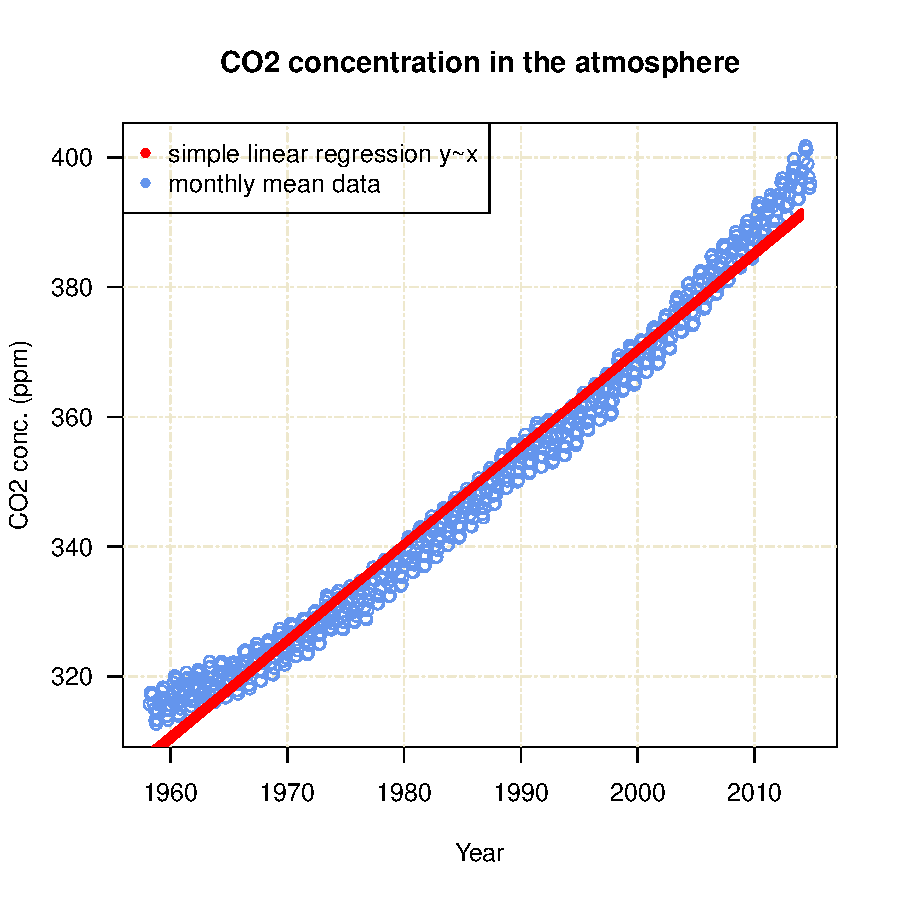
\includegraphics{alleselena-plotorigin}
\end{figure}

The plot ~/ref{plotorigin} can be used to identify potential outliers in the dataset which could possibly bias the future model.  Due to the plot we can see, that we don't have any outliers and we can go on, having a look at the added simple poly-1 linear regression. The lm is not accurate in fitting the dataset. There are missing a lot of model predictors.

In table ~/ref{stde_lm}  the standard errors of the linear regression are small.  One possible attribute of a time series is, that the residuals are serially correlated. With this autocorrelation, the standard errors shown in the lm would be underestimated, thus far too small.  Subsequently, the resulting significance  from the t-test ( p-value) is lower than it should be. In our case this would mean, that CO2 concentrations are rising significantly and that we have a enormous problem with our atmospheric composition. 

\begin{Schunk}
\begin{Sinput}
> xtable(summary(datalm)$coef)
\end{Sinput}
% latex table generated in R 3.1.1 by xtable 1.7-4 package
% Thu Nov 27 21:02:33 2014
\begin{table}[ht]
\centering
\begin{tabular}{rrrrr}
  \hline
 & Estimate & Std. Error & t value & Pr($>$$|$t$|$) \\ 
  \hline
(Intercept) & -2618.56 & 16.98 & -154.23 & 0.00 \\ 
  year & 1.49 & 0.01 & 174.86 & 0.00 \\ 
   \hline
\end{tabular}
\end{table}\end{Schunk}


\subsection{Dataset Transformation}
It is essential to transform your dataset into a timeseries (ts) if you seek for an accurate and extensive analysis of the data.
\noindent The data stored as a dataframe needs to be transformed with the important columns into the class of a time series to continue working on it properly. If you have monthly data you have to set the deltat of the function ts() to deltat=1/12 describing the sampling period parts between successive values xt and xt+1. Your time series should somehow look like table 1.\\
\noindent \textbf{Original Data}\\
\begin{Schunk}
\begin{Sinput}
> xtable(head(data), caption="Original CO2-Data")
\end{Sinput}
% latex table generated in R 3.1.1 by xtable 1.7-4 package
% Thu Nov 27 21:02:33 2014
\begin{table}[ht]
\centering
\begin{tabular}{rrr}
  \hline
 & year & co2 \\ 
  \hline
1 & 1958.21 & 315.71 \\ 
  2 & 1958.29 & 317.45 \\ 
  3 & 1958.38 & 317.50 \\ 
  4 & 1958.46 & 317.10 \\ 
  5 & 1958.54 & 315.86 \\ 
  6 & 1958.62 & 314.93 \\ 
   \hline
\end{tabular}
\caption{Original CO2-Data} 
\end{table}\end{Schunk}
\noindent \textbf{Transformation}\\
\begin{Schunk}
\begin{Sinput}
> yourts=ts(co2, c(1958,3),c(2014,10), deltat=1/12)
> class(yourts)
\end{Sinput}
[1] "ts"\begin{Sinput}
> time = time(yourts)
> 
\end{Sinput}
\end{Schunk}
%<<results=tex, echo=FALSE, print=TRUE >>=
%print(xtable(yourts, digits=2, label="yourts",caption="Your time series for monthly mean data"), size="\\tiny")
%@
%\pagebreak
\subsection{Time-Series Visualization}%------------------------------------------------------------------------------------
It is  also helpful to get a quick overview of the time series class of our data with some plots.\\ 
The original data and the time series data are the same, thus it is important to have a different class for further working on it. \\
\subsubsection{Time-Series Plot}
\begin{figure}[H]
\centering
\begin{Schunk}
\begin{Sinput}
> par(mfrow=c(1,1))
> plot(time, co2,type="n",las=1, xlab="Year", ylab="CO2 conc. (ppm)",
         main="CO2 concentration in the atmosphere")
> grid (NULL,NULL, lty = 6, col = "cornsilk2")
> points(yourts, col="cornflowerblue" )
> lines(year, co2, col="red")
> legend("topleft",c("time series", "monthly mean raw data"),
 pch=c(20,20), col=c("red", "cornflowerblue"))
\end{Sinput}
\end{Schunk}
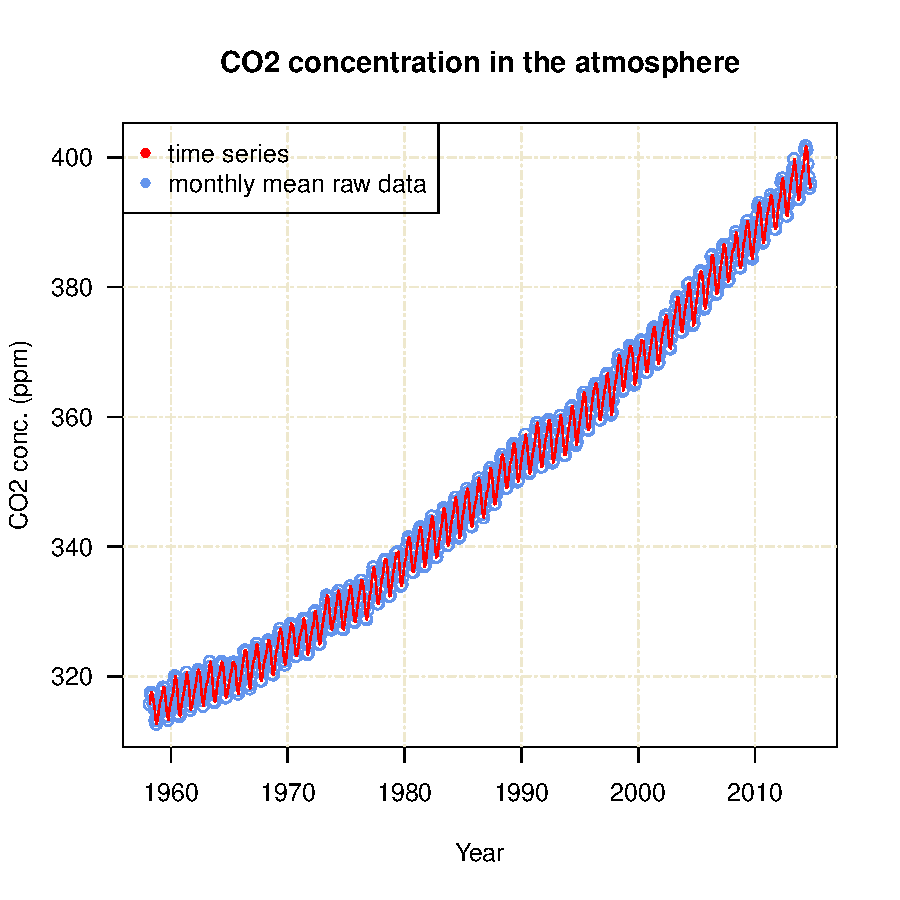
\includegraphics{alleselena-fig1visualize}
\caption{Visualization of the CO2 Concentrations}
\label{fig1visualize}
\end{figure}


%\pagebreak
\subsubsection{ACF, PACF, SPECTRUM}
\noindent   2. Correlogram:  The correlogram is divided by three different functions all depicting important information on the autocorrelation and the cyclic component of our time series.  The problem we face with time series is the possible violation of independence assumption of a model, meaning that the SE is possibly too small. If the data are equally spaced in time,  the autocorrelation functions can be used to investigate residual  correlations in the model errors. The correlograms produce lags which are either within the CI or outter CI. If a lag is bigger than the CI, you need to include the lag as a order of autocorrelation in your AR or\- and MA terms which are needed in the following models. 


\begin{figure}[H]
\centering
\begin{Schunk}
\begin{Sinput}
> acf(co2, xlab="", main = "")
\end{Sinput}
\end{Schunk}
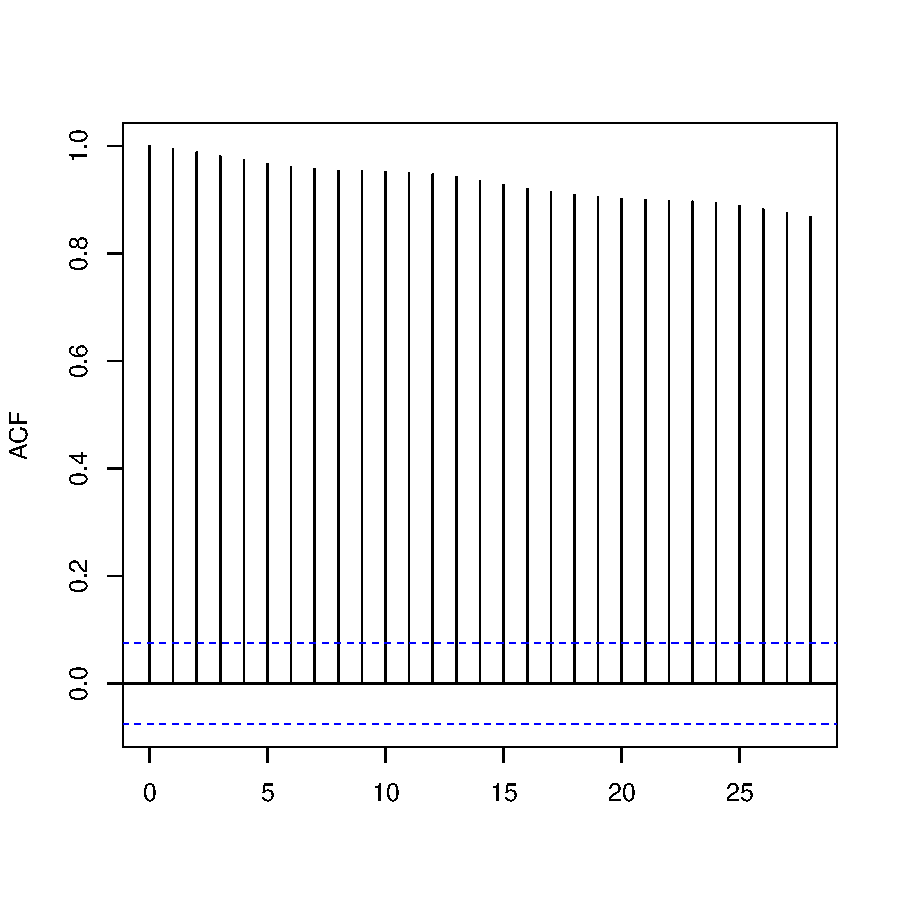
\includegraphics{alleselena-ACF_co2}
 \caption{ACF of CO2 Concentrations}
\label{correlogramlm}
\end{figure}


\begin{figure}[H]
\centering
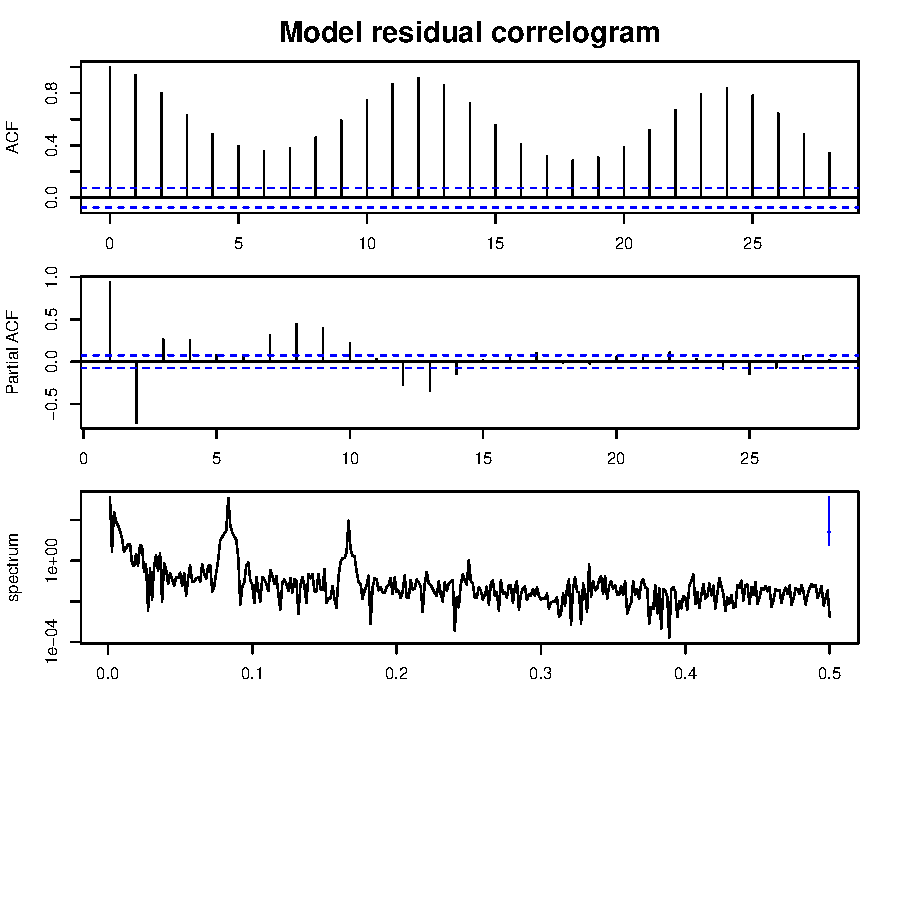
\includegraphics{alleselena-correlogramres}
\caption{Correlogram of residuals of lm}
\label{correlogramlm}
\end{figure}

\noindent   \textbf{ACF}:  The autocorrelation function ACF() is one option producing a  plot of coefficients of correlation between your time series and lags of itself.   If you have a correlation at lag 1 and one at lag 2, the first correlation is reproduced to the second and so on to higher-order lags. This pattern, similar to the one in plot ~/ref{ACF_co2} is like a flow-on effect from the dependence at lag 1, which would be typical for an autoregressive process. 
	
\textbf{	The PACF ( partial ACF)} is the accumulation of correlations between 2 variables excluding the correlation explained by their common correlation. It is not explained in the lower-order-lags. If you have correlations at lag 1 and at lag 2, the PACF computes the difference between the actual correlation at lag 2 and the expected correlation if reprdocution of the correlation at lag 1. 
	
	In our correlogram, the lag \emph{p=1}  included  as a autoregressive order in the model will capture already a lot of the correlation structure. 
	
	The \textbf{spectrum} will be the third function used to check for possible correlation structures  showing the spectral density of the time series over frequencies. If a local maximum occurs,  \emph{1/(local max.)} can be used as equation to pick a possible periodic term. For our data we have a spectrum max at 0.75, meaning there might be a 12 * periodic cycle ( 12 months = 1 year) . 
	
	The residuals in a time series are serially correlated. The ACF is waving and decreases only slowly, which would be an identification of non-stationarity. We stop here all following diagnostic tests due to the clear autocorrelation in our data and investigate the different components of our time series. 

\section{Decomposition of Time Series}%-----------------------------------------------------------------------------------------------------
As described in the ~/ref{Introduction} , a time series consists usually of 3 components; a trend component, an irregular (random) component and (if it is a seasonal time series) a seasonal component. 



Figure  ~/ref{seasadj} depicts the comparison between the data with and without the seasonal fluctuation. In some cases it might be handy to have the model without the seasonal fluctuations to empahize the trend and the random part or to compute means more acurately.  
 
\subsection{Decomposing Seasonal Data}%----------------------------------------------------------------------------------------------------
\noindent We can decompose the ts and plot these components:
\begin{figure}[H]
\centering
\begin{Schunk}
\begin{Sinput}
> plot(decompose(yourts))
\end{Sinput}
\end{Schunk}
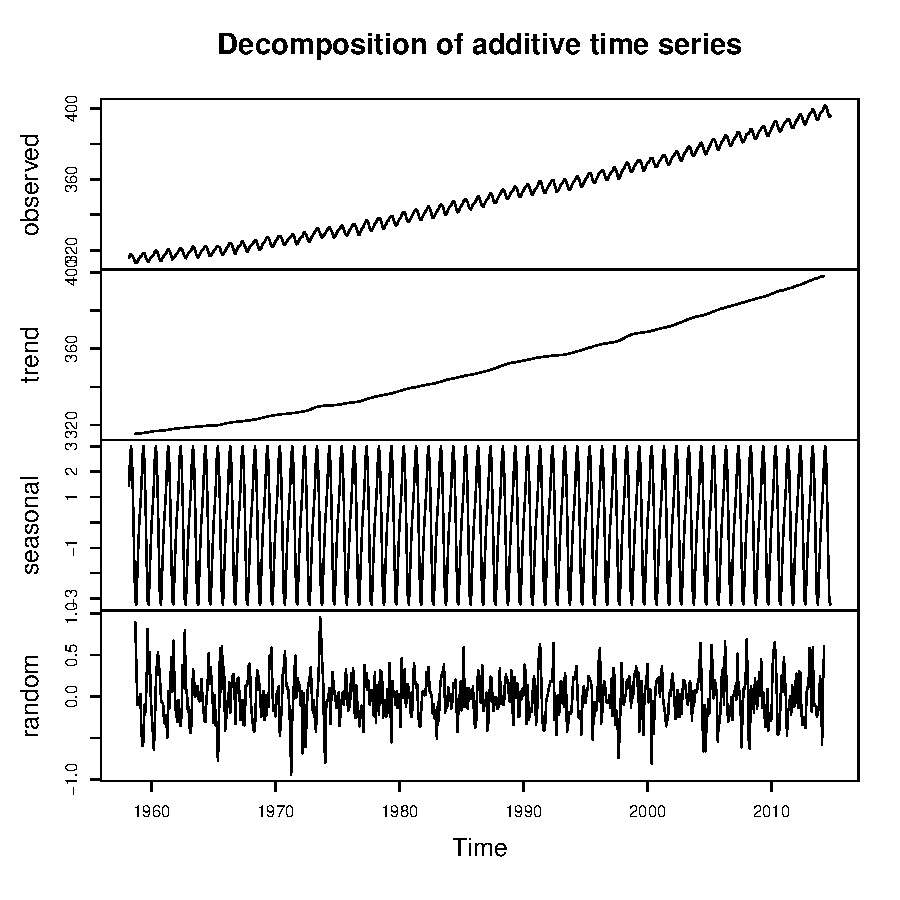
\includegraphics{alleselena-decompose}
\caption{Decomposition of the CO2 Time Series}
\end{figure}


\noindent We can see each component with:
\begin{Schunk}
\begin{Sinput}
> yourts_components<- decompose(yourts)
\end{Sinput}
\end{Schunk}
\begin{Schunk}
\begin{Sinput}
> yourts_components$seasonal
\end{Sinput}
\end{Schunk}


\begin{figure}[H]
\centering
\begin{Schunk}
\begin{Sinput}
> #we can see the trend for the first year:
> par(mfrow=c(1,2))
> ts.plot(yourts_components$seasonal[1:12])
> ts.plot(aggregate(yourts_components$seasonal))
\end{Sinput}
\end{Schunk}
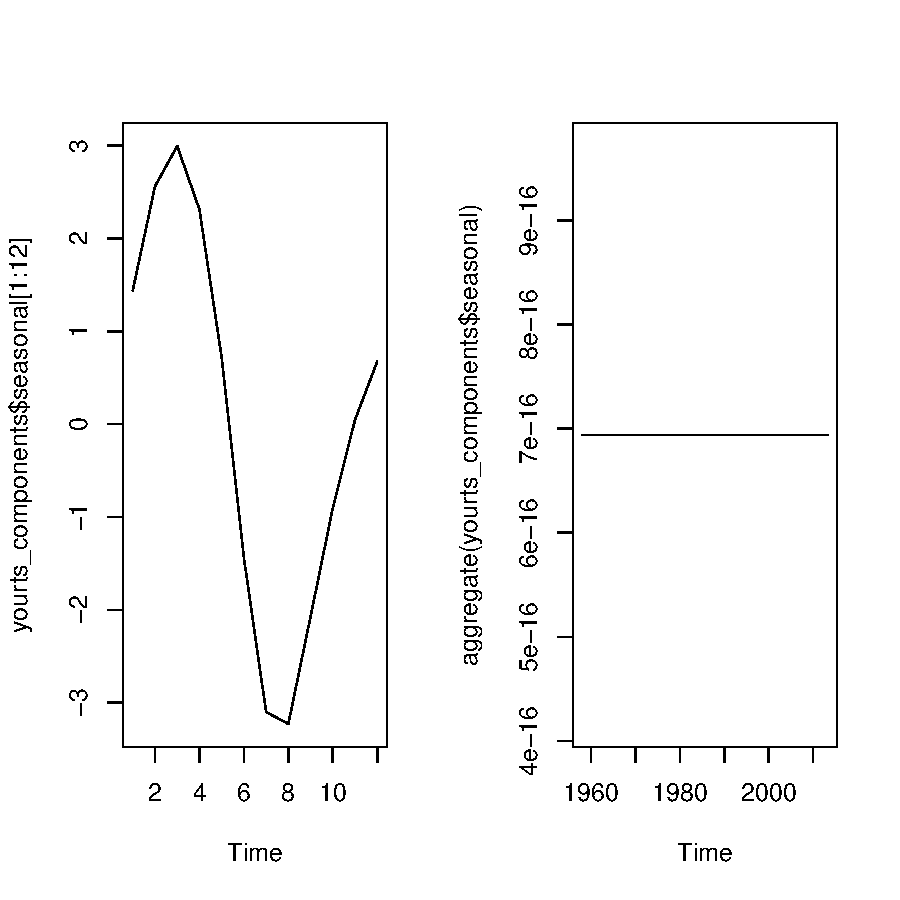
\includegraphics{alleselena-seascomp}
\caption{The seasonal component across the time}
\label{seascomp}
\end{figure}

In the figure ~/ref{seascomp} , the monthly and annual component are depicted, respectively. It seems that our seasonal component is positive in the first half of the year ( month 1-6) and is negative in the second half of the year. The annual seasonal component is though constant within our time series. This assumes that we can fully include the seasonal term in an additive model without adding additional random noise to it or biasing the long-term trend. 

\begin{figure}[H]
\centering
\begin{Schunk}
\begin{Sinput}
> yourts_seasonallyadjusted <- yourts - yourts_components$seasonal
> par(mfrow=c(1,2))
> plot(yourts, main="TS with seasonal fl.", las=1)
> plot(yourts_seasonallyadjusted, las=1, main="removed seasonal fluctuation")
\end{Sinput}
\end{Schunk}
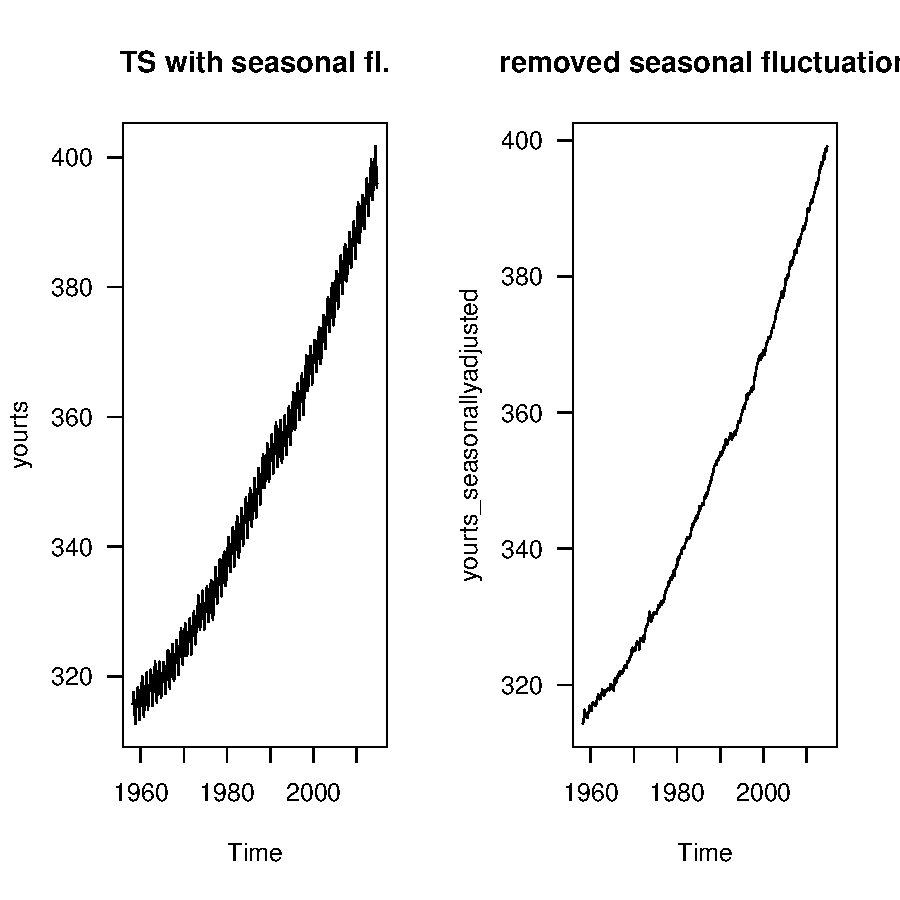
\includegraphics{alleselena-seasadj}
\caption{Comparison of seasonal vs. seasonally adjusted model}
\label{seasadj}
\end{figure}

\noindent Figure  ~/ref{seasadj} depicts the comparison between the data with and without the seasonal fluctuation. In some cases it might be handy to have the model without the seasonal fluctuations to empahize the trend and the random part or to compute means more acurately.  


\section{Modelling the time series}
In this tutorial, the aim of the analysis of a seasonal time series is mainly  to generate forecasts  and make the time series stationary. For this, we need to define a model which has all the needed components of the time series. 

\begin{Schunk}
\begin{Sinput}
> adftable <- function(x) {
 stat.res =signif(adf.test(x)$p.value);
 stat.alt = adf.test(x)$alternative;
 c1 = cbind( stat.res, stat.alt);
 c2 = c("stationarity of time series",
         "alternative");
 matrixsmall = as.matrix(c1,c2);
 colnames(matrixsmall)= c("stationarity p-value",
         "alternative");
 return ( matrixsmall)
 }
\end{Sinput}
\end{Schunk}

After looking at the simple linear regression datalm, we were facing some serious problems with our model. To be sure about the stationarity we run an adf.test() giving p-value of .... 

\begin{Schunk}
\begin{Sinput}
> xtable(adftable(yourts), main="Adf test for stationarity")
\end{Sinput}
\begin{Soutput}
% latex table generated in R 3.1.1 by xtable 1.7-4 package
% Thu Nov 27 21:02:34 2014
\begin{table}[ht]
\centering
\begin{tabular}{rll}
  \hline
 & stationarity p-value & alternative \\ 
  \hline
1 & 0.928016 & stationary \\ 
   \hline
\end{tabular}
\end{table}
\end{Soutput}
\end{Schunk}

Also we need a model, which is covering the serial correlation of our residuals. The ACF; PACF and the spectrum gives us certainty that there is some autocorrelation and seasonal fluctuation. glm() cannot allow for autocorrelation. The generalized least squares  model is one option that can be used to allow for autocorrelation of standard errors and unequal variances. 


\subsection{Analysis of Seasonal Data with GLS}

The generalized least squares  model is one option that can be used to allow for autocorrelation of standard errors and unequal variances. 
\linebreak

In the gls() we have different options to choose for our covariance structure. Because our data is not spatially correlated we are not discussing spatial autocorrelation here.\\

For temporal correlation we have five options:
\begin{enumerate}
\item corAR1: in ACF exponential decreasing values of correlation with time distance\\
\item corARMA: either autoregressive order or moving average order or both\\
\item corCAR1: continuous time ( time index does nto have to be integers)\\
\item corCompSymm: correlation does not decrease with higher distance\\
\item corSymm: general correlation only for few observations only, often overparameterized\\
\end{enumerate}



Our first gls() model accounts for the AR1, which is clearly visible in the PACF. 
Our lag 1 is the lag computed from the linear regression ACF.

\begin{Schunk}
\begin{Sinput}
> data.glsAR = gls(yourts ~ time,cor= corAR1(acf(resid(datalm))$acf[2]))
> save(data.glsAR, file="data.glsAR.RData")
\end{Sinput}
\end{Schunk}

\begin{Schunk}
\begin{Sinput}
> load("data.glsAR.RData")
\end{Sinput}
\end{Schunk}


\begin{figure}[H]
\centering
\begin{Schunk}
\begin{Sinput}
> par(mfrow=c(1,2))
> acf(data.glsAR$residuals)
> pacf(data.glsAR$residuals)
\end{Sinput}
\end{Schunk}
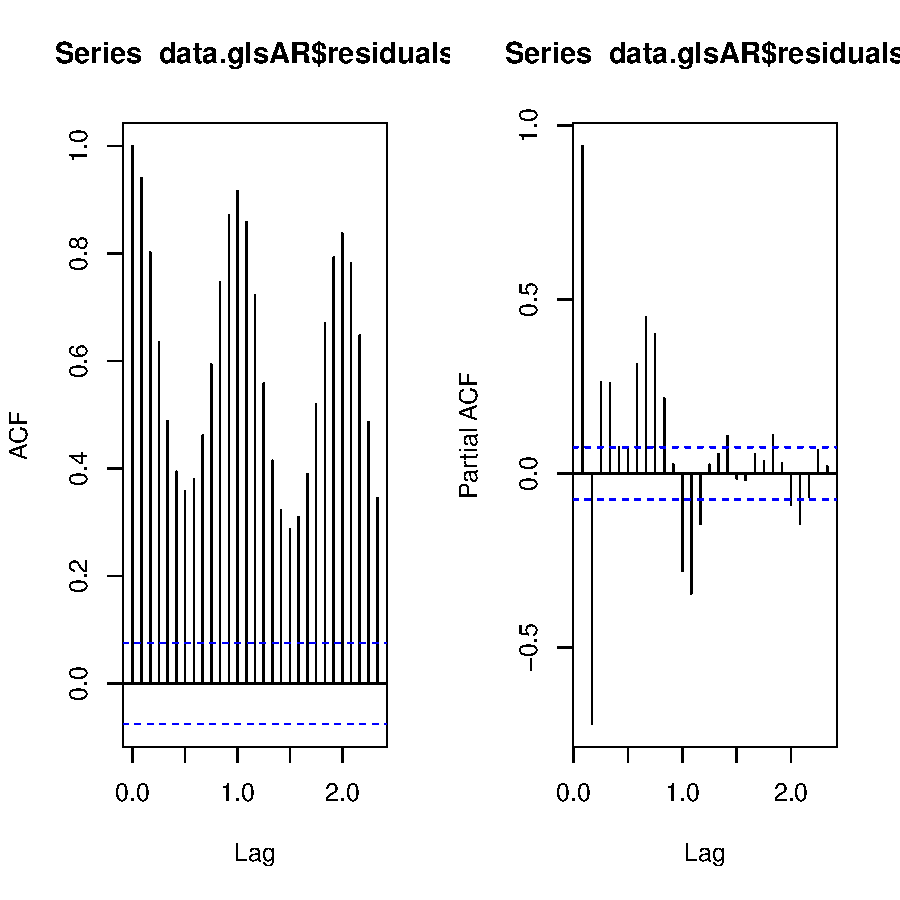
\includegraphics{alleselena-correlogram}
\caption{Correlogram of GLS  with AR(1) structure}
\label{corglsAR}
\end{figure}

We still face a lot of problems with the first GLS model only including 1 auto regressive order. 
One option is to allow the AR to use more parameters and/or to include a moving average or error variance to the model. This can be handled via the corARMA. We tried 2 versions, one with 1 lag and 1 moving average, the other with 2 lags and 2 moving averages.
The 0.2 are starting values for Phi, which are in the modelling process optimized.
The next models are thus:
\begin{Schunk}
\begin{Sinput}
> dataglsARMA10 = gls ( yourts ~ time, cor = corARMA (p=1, q=0 ))
> dataglsARMA11 = update (dataglsARMA10, cor=corARMA(p=1, q=1))
> dataglsARMA12 = update (dataglsARMA10, cor=corARMA(p=1, q=2))
> dataglsARMA22 = update (dataglsARMA10, cor=corARMA(p=2, q=2))
> dataglsARMA21 = update (dataglsARMA10, cor=corARMA(p=2, q=1))
> save(dataglsARMA10, file="dataglsARMA10.RData")
> save(dataglsARMA11, file="dataglsARMA11.RData")
> save(dataglsARMA12, file="dataglsARMA12.RData")
> save(dataglsARMA22, file="dataglsARMA22.RData")
> save(dataglsARMA21, file="dataglsARMA21.RData")
> 
\end{Sinput}
\end{Schunk}

\begin{Schunk}
\begin{Sinput}
> load(file="dataglsARMA10.RData")
> load( file="dataglsARMA11.RData")
> load( file="dataglsARMA12.RData")
> load( file="dataglsARMA22.RData")
> load( file="dataglsARMA21.RData")
\end{Sinput}
\end{Schunk}

The AIC (Akaike Information Criterion) is used to compare the different models. The smaller the AIC value, the better fits the model to the original dataset.  
To compare all the models we use anova and the best model is so far the dataglsARMA22 with the lowest AIC and significantly better than the ARMA(2,1), which is itself not better than the ARMA(1,2), but this is better than the previous 2 models. 

\begin{Schunk}
\begin{Sinput}
> anova(dataglsARMA10,dataglsARMA11,dataglsARMA12,dataglsARMA21,dataglsARMA22)
\end{Sinput}
\begin{Soutput}
              Model df      AIC      BIC     logLik   Test
dataglsARMA10     1  4 2189.575 2207.651 -1090.7874       
dataglsARMA11     2  5 1760.113 1782.709  -875.0567 1 vs 2
dataglsARMA12     3  6 1587.709 1614.824  -787.8545 2 vs 3
dataglsARMA21     4  6 1549.076 1576.191  -768.5380       
dataglsARMA22     5  7 1495.348 1526.982  -740.6742 4 vs 5
               L.Ratio p-value
dataglsARMA10                 
dataglsARMA11 431.4614  <.0001
dataglsARMA12 174.4045  <.0001
dataglsARMA21                 
dataglsARMA22  55.7275  <.0001
\end{Soutput}
\end{Schunk}

\begin{Schunk}
\begin{Sinput}
> diagnostics(dataglsARMA22)
\end{Sinput}
\begin{Soutput}
     normality    stat.res   stat.res.alt
[1,] "1.8632e-08" "0.928016" "stationary"
     autocorr            indep
[1,] "0.111186713059271" "0"  
\end{Soutput}
\end{Schunk}

\begin{figure}[H]
\centering
\begin{Schunk}
\begin{Sinput}
> plot(datalm, which = 1:1)
> #well spread is already smaller of variances
\end{Sinput}
\end{Schunk}
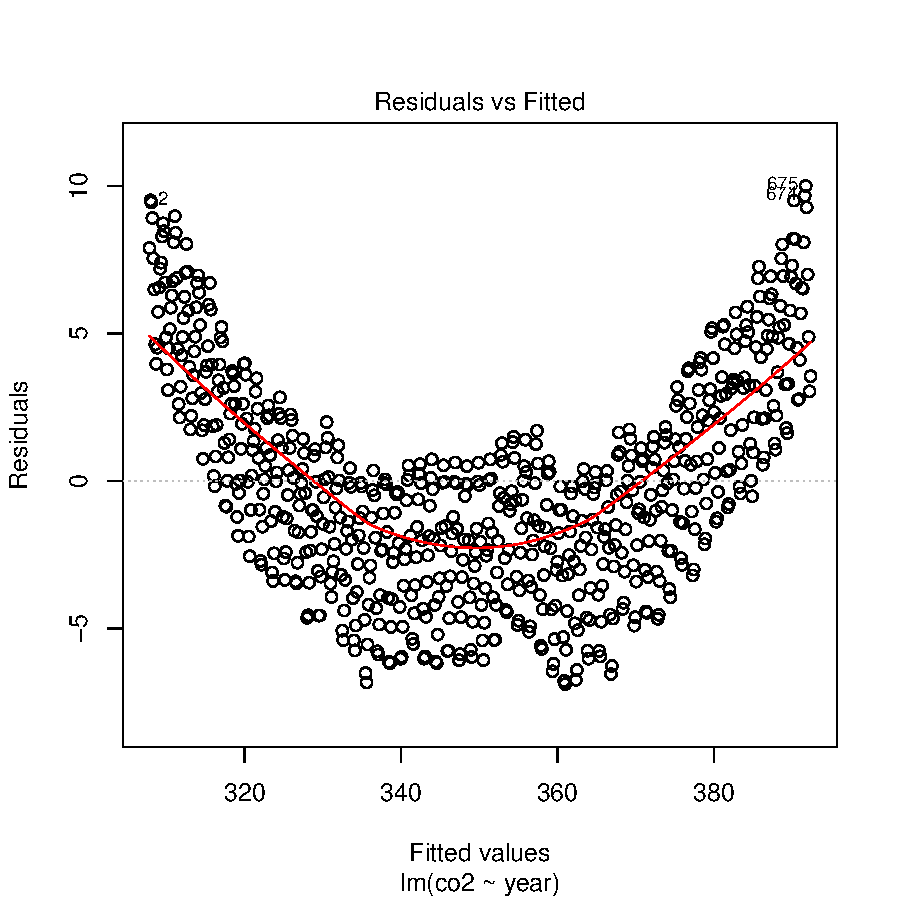
\includegraphics{alleselena-residual}
\caption{Residuals fitted vs. observed in LM}
\label{residual}
\end{figure}\\

\begin{figure}[H]
\centering
\begin{Schunk}
\begin{Sinput}
> plot(dataglsARMA22)
\end{Sinput}
\end{Schunk}
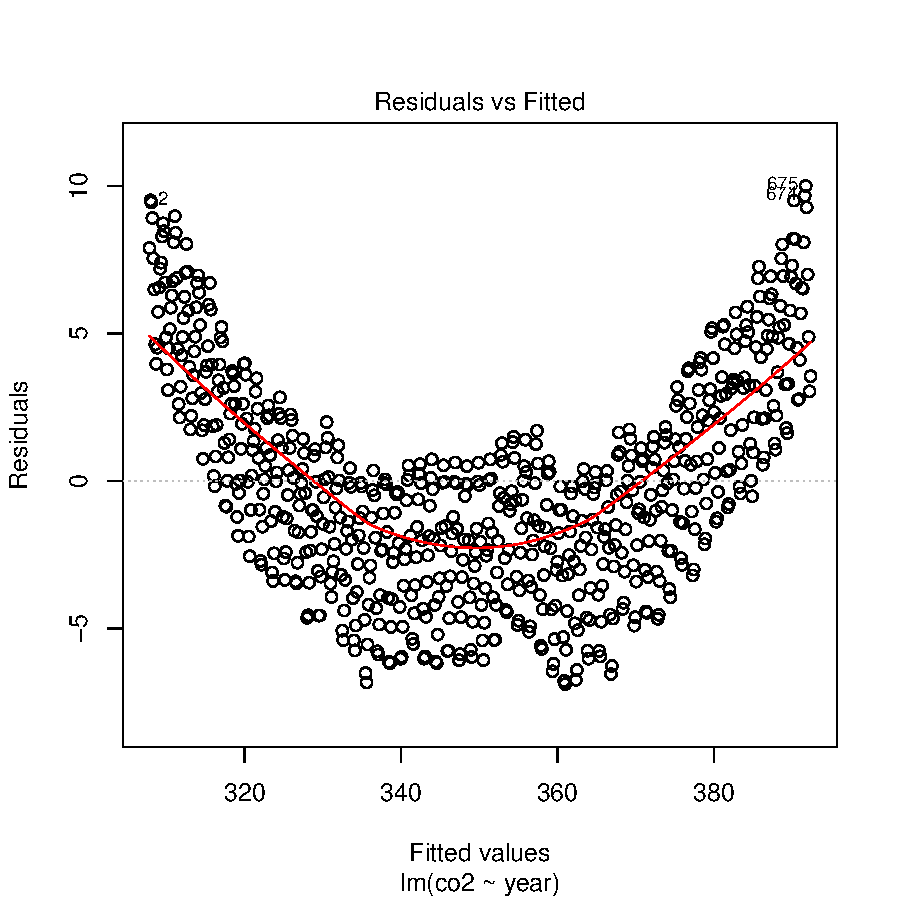
\includegraphics{alleselena-residual}
\caption{Residuals fitted vs. observed in GLS}
\label{residual}
\end{figure}\\

\noindent Now, the best correlation structure seems to be selected, however the seasonal component is still missing. We need to include that in a simple version: 


\begin{Schunk}
\begin{Sinput}
> seas = cycle(yourts)
> dataseasongls = gls(yourts ~ time + factor(seas), cor=corARMA(c(0.2,0.2,0.2,0.2),p=2, q=2)) #use bestmodel corStruct
> save(dataseasongls, file="dataseasongls.RData")
\end{Sinput}
\end{Schunk}

\begin{Schunk}
\begin{Sinput}
> load("dataseasongls.RData")
\end{Sinput}
\end{Schunk}

\begin{figure}[H]
\centering
\begin{Schunk}
\begin{Sinput}
> par(mfrow=c(2,1))
> acf(dataseasongls$residuals)
> pacf(dataseasongls$residuals)
\end{Sinput}
\end{Schunk}
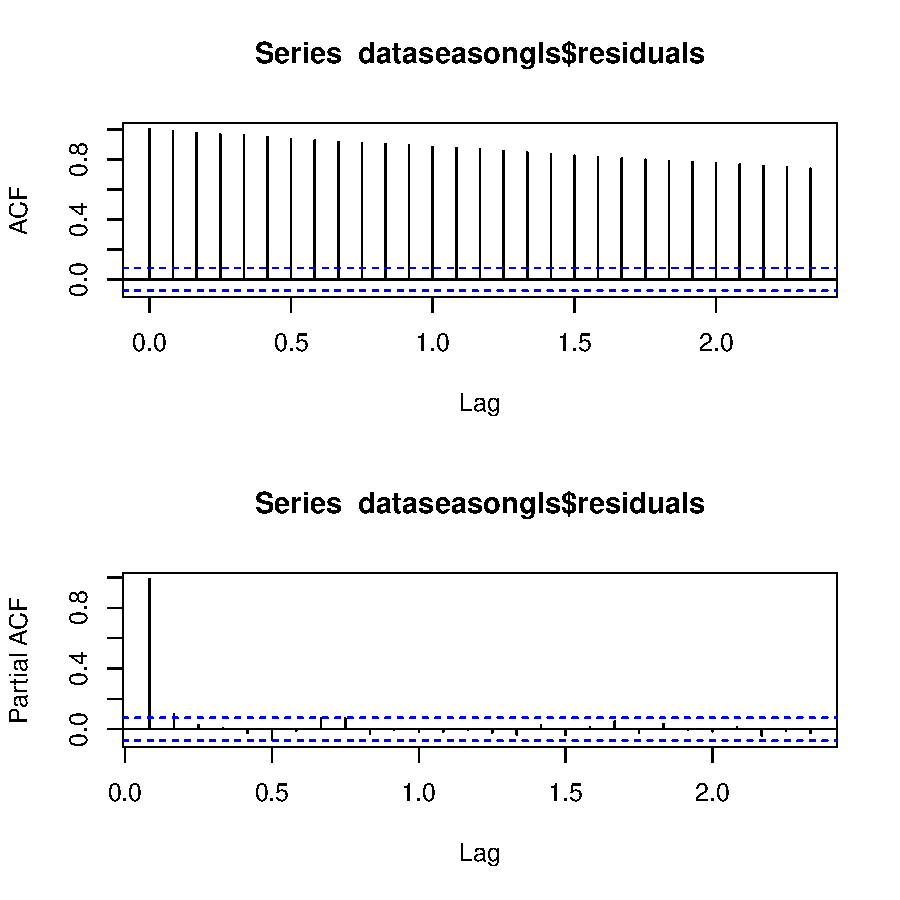
\includegraphics{alleselena-corseas}
\caption{Correlogram of season included model}
\label{corseas}
\end{figure}


\begin{figure}[H]
\centering
\begin{Schunk}
\begin{Sinput}
> par(mfrow=c(1,1))
> plot(dataseasongls$residuals,ylab="Residuals", xlab="Year", las=1, type="p", col="cornflowerblue", main="Residuals of dataseasongls over time") 
> 
\end{Sinput}
\end{Schunk}
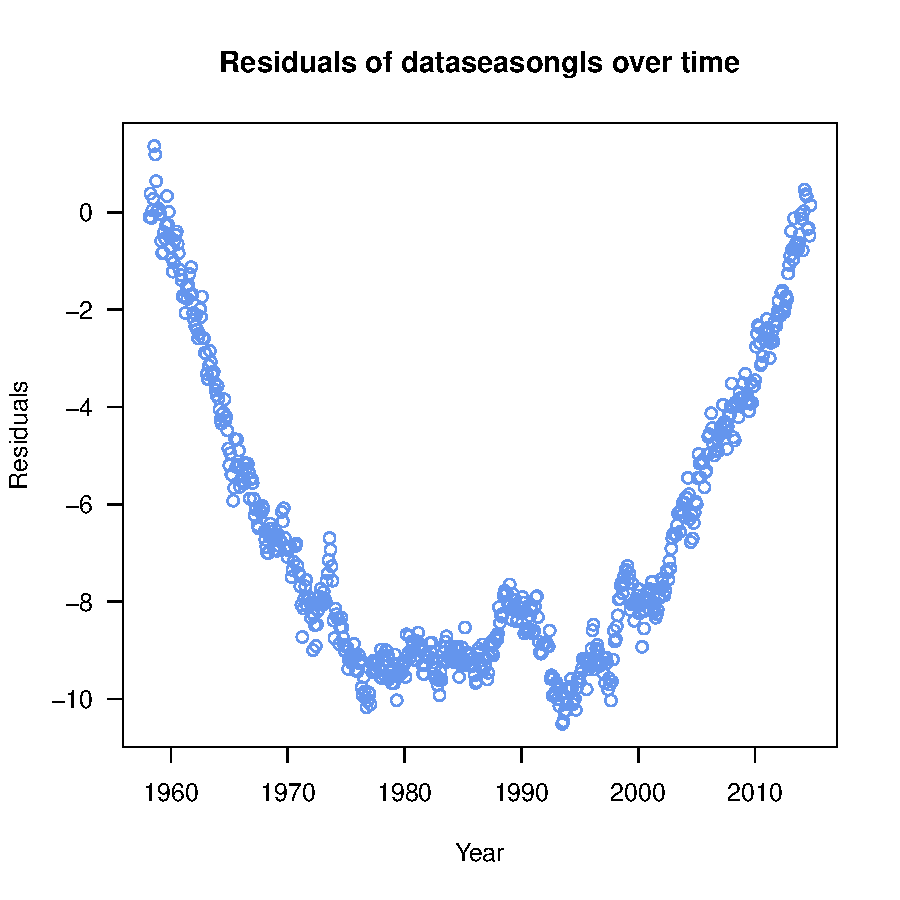
\includegraphics{alleselena-resseas}
\caption{Residuals of season included model}
\label{resseas}
\end{figure}

The problem with anova.gls is that it cannot compare gls() with different fixed effects. The added seasonal term is such an effect, thus the anova does not work here. We need to compare the AIC by hand and see an improvement. 


\begin{Schunk}
\begin{Sinput}
> AIC(dataglsARMA22)
\end{Sinput}
[1] 1495.348\begin{Sinput}
> AIC(dataseasongls)
\end{Sinput}
[1] 401.2934\begin{Sinput}
> #write function choosing best model 
\end{Sinput}
\end{Schunk}

\begin{figure}[H]
\centering
\begin{Schunk}
\begin{Sinput}
> ts.plot(cbind(yourts, dataglsARMA22$fitted,
               dataseasongls$fitted),
         lty=1:2, col=c(1,2,3), 
         main="Compare mean monthly data with gls model")
> legend(1960,400,c("Original",
                   "Fitted for Autocorrelation",
                   "Fitted for Seasonality"),
        col=c(1,2,3),lty=c(1, 2,3))
\end{Sinput}
\end{Schunk}
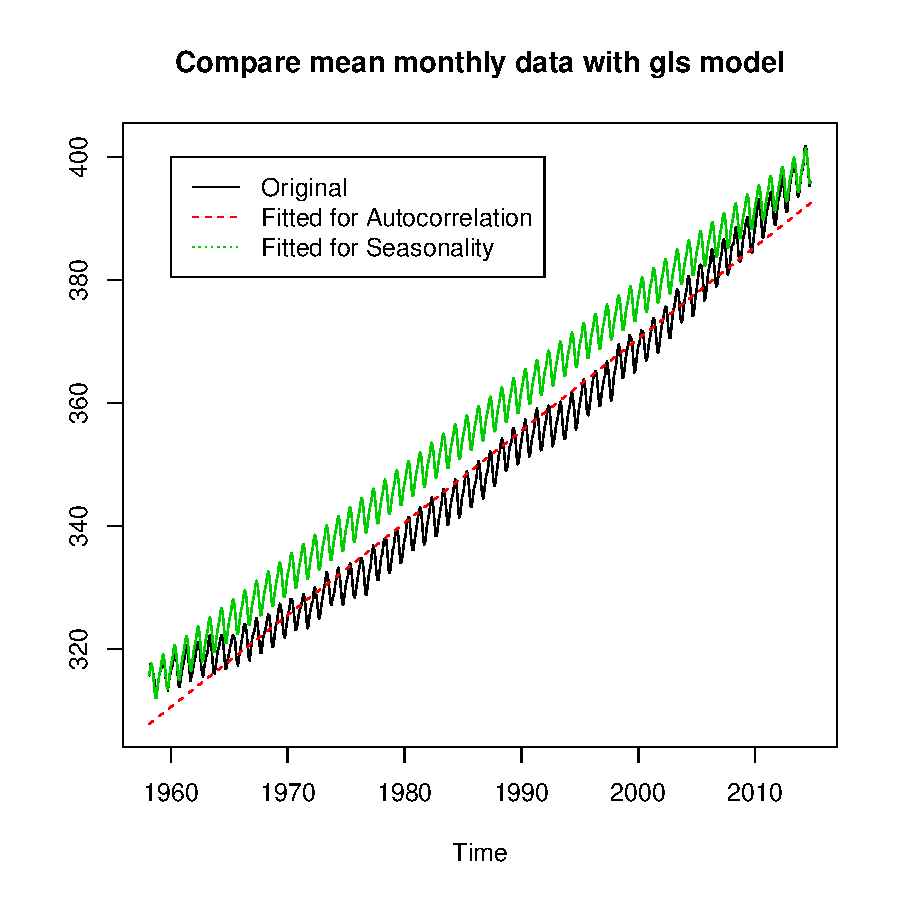
\includegraphics{alleselena-036}
\caption{Comparison of season included model and only autocorr. included model}
\label{compseas2}
\end{figure}

In the figure ~\ref{compseas2} you see the options we were trying so far to come closer to our adequate model. One option is the ARMA22 GLS including autocorrelation, the second option is to include the seasonality by adding a fixed effect (factor(season)) to our gls. 
The seasonal effect inclusion clearly improves our model. But the original data is slightly curved and we see in plot ~/ref{resseas} that the residuals get bigger as soon as the bending of the original data sets in and flatten again as soon as the model was close to the end point in 2014. \\

We should include a quadratic term and generalize our seasonality with a continuous sin-cos wave:\\

\begin{Schunk}
\begin{Sinput}
> SIN = COS = matrix(nr=length(yourts), nc=6)
> for (i in 1:6) {
   COS[,i] <- cos(2*pi*i*time(yourts))
   SIN[,i] <- sin(2*pi*i*time(yourts)) 
 }
> time = time(yourts)
\end{Sinput}
\end{Schunk}
#also was done by hand in self writing seasonality removal above
Thus we do not know how many changes in the wave we need to include, we include 6 changes in the wave to be certain that the next model can follow the best wave option. 

Before this, add a quadratic term ( polynomial (x,2)), x = years) will change the linear regression by including a slight bending in the fitted values over time, which we saw in the original data. 


\begin{Schunk}
\begin{Sinput}
> harmonizedgls<-gls(yourts ~ time + I(time^2) +
                     COS[,1]+SIN[,1]+COS[,2]+SIN[,2]+
                     COS[,3]+SIN[,3]+COS[,4]+SIN[,4]+
                     COS[,5]+SIN[,5]+COS[,6]+SIN[,6],
                   corr=corAR1(acf(dataseasongls$residuals)$acf[2]))
> save(harmonizedgls, file="harmonizedgls.RData")
> harmonizedARMAgls<-gls(yourts ~ time + I(time^2) +
                       COS[,1]+SIN[,1]+COS[,2]+SIN[,2]+
                       COS[,3]+SIN[,3]+COS[,4]+SIN[,4]+
                       COS[,5]+SIN[,5]+COS[,6]+SIN[,6]
                     , cor=corARMA(p=2, q=2))
> save(harmonizedARMAgls, file="harmonizedARMAgls.RData")
\end{Sinput}
\end{Schunk}

\begin{Schunk}
\begin{Sinput}
> load("harmonizedARMAgls.RData")
> load("harmonizedgls.RData")
\end{Sinput}
\end{Schunk}

\begin{Schunk}
\begin{Sinput}
> AIC(harmonizedgls) #even smaller 
\end{Sinput}
\begin{Soutput}
[1] 396.86
\end{Soutput}
\begin{Sinput}
> AIC(harmonizedARMAgls) #even smaller 
\end{Sinput}
\begin{Soutput}
[1] 360.4082
\end{Soutput}
\begin{Sinput}
> xtable(anova(harmonizedgls,harmonizedARMAgls))
\end{Sinput}
\begin{Soutput}
% latex table generated in R 3.1.1 by xtable 1.7-4 package
% Thu Nov 27 21:02:36 2014
\begin{table}[ht]
\centering
\begin{tabular}{rlrrrrrlrr}
  \hline
 & call & Model & df & AIC & BIC & logLik & Test & L.Ratio & p-value \\ 
  \hline
harmonizedgls & gls(model = yourts \~{} time + I(time\verb|^|2) + COS[, 1] + SIN[, 1] +     COS[, 2] + SIN[, 2] + COS[, 3] + SIN[, 3] + COS[, 4] + SIN[,     4] + COS[, 5] + SIN[, 5] + COS[, 6] + SIN[, 6], correlation = corAR1(acf(dataseasongls\$residuals)\$acf[2])) &   1 &  17 & 396.86 & 473.36 & -181.43 &  &  &  \\ 
  harmonizedARMAgls & gls(model = yourts \~{} time + I(time\verb|^|2) + COS[, 1] + SIN[, 1] +     COS[, 2] + SIN[, 2] + COS[, 3] + SIN[, 3] + COS[, 4] + SIN[,     4] + COS[, 5] + SIN[, 5] + COS[, 6] + SIN[, 6], correlation = corARMA(p = 2,     q = 2)) &   2 &  20 & 360.41 & 450.40 & -160.20 & 1 vs 2 & 42.45 & 0.00 \\ 
   \hline
\end{tabular}
\end{table}
\end{Soutput}
\end{Schunk}



\begin{figure}[H]
\centering
\begin{Schunk}
\begin{Sinput}
> par(mfrow=c(1,1))
> ts.plot(cbind(yourts,dataseasongls$fitted, harmonizedARMAgls$fitted), col=c(1,2,3),
         main="Compare mean monthly data with gls model")
> legend(1960,400,c("Original", "Included seasonality ",
                   "Polynm. + seasonality"),col=c(1,2,3), pch=c(20,20,20))
\end{Sinput}
\end{Schunk}
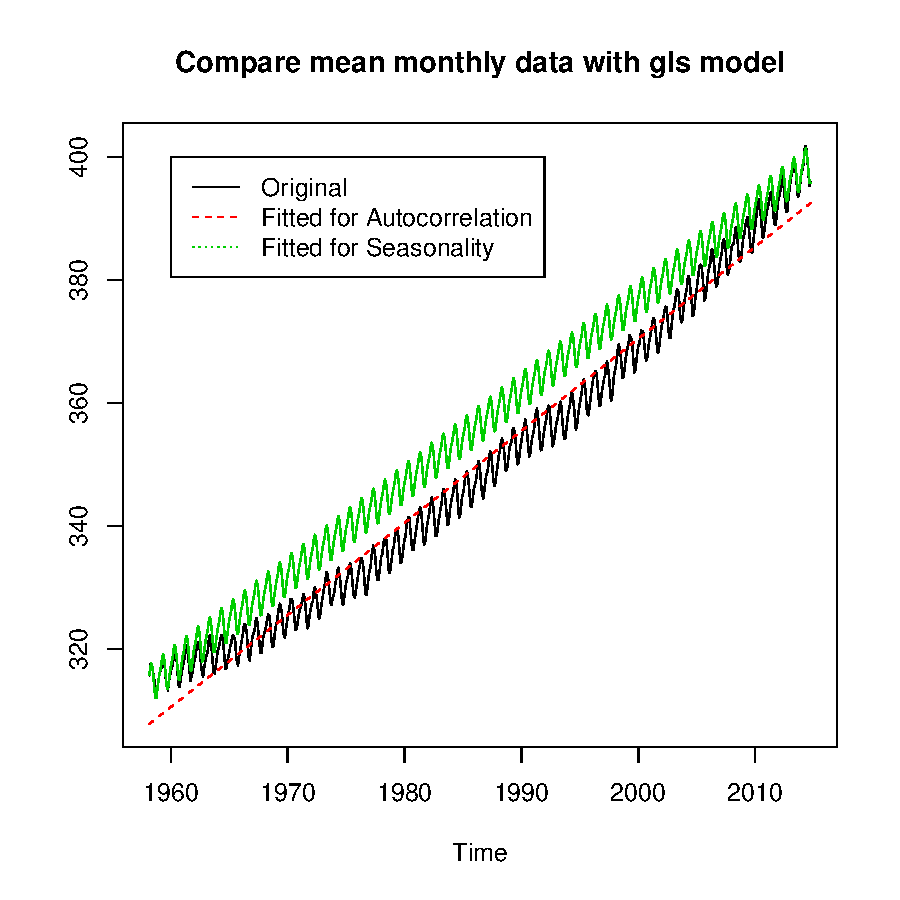
\includegraphics{alleselena-041}
\caption{Comparison of season and quadr. term included model}
\label{compq}
\end{figure}

\linebreak
residuals compare\\
\begin{figure}[H]
\centering
\begin{Schunk}
\begin{Sinput}
> plot(datalm, which = 1:1)
\end{Sinput}
\end{Schunk}
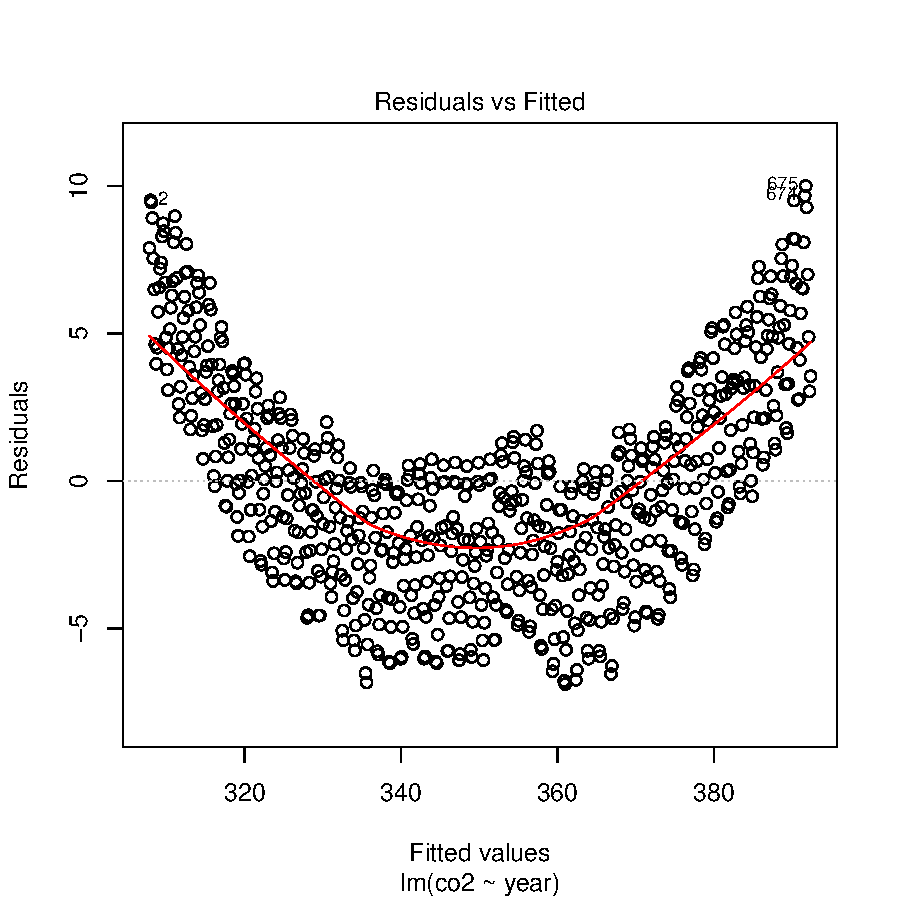
\includegraphics{alleselena-042}
\caption{Residuals fitted vs. obs. values}
\label{comparison_finalgls1}
\end{figure}

\begin{figure}[H]
\centering
\begin{Schunk}
\begin{Sinput}
> plot(dataglsARMA22)
\end{Sinput}
\end{Schunk}
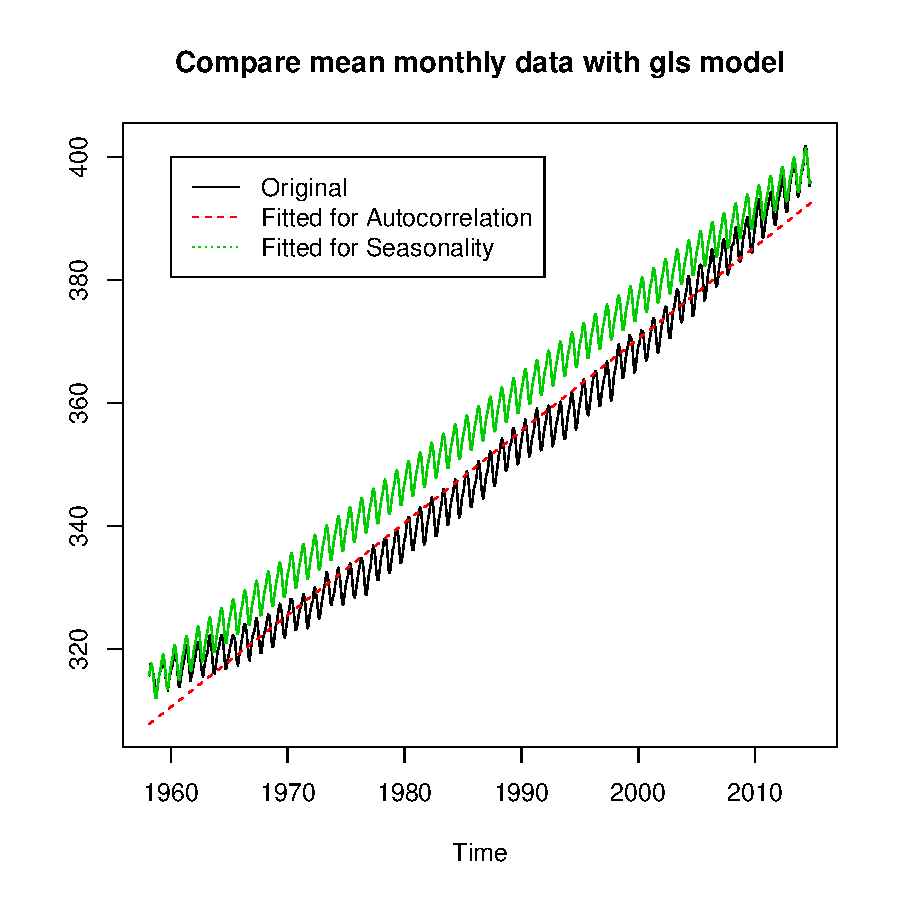
\includegraphics{alleselena-043}
\caption{Residuals fitted vs. obs. values ARMA}
\label{comparison_finalgls2}
\end{figure}

\begin{figure}[H]
\centering
\begin{Schunk}
\begin{Sinput}
> plot(harmonizedARMAgls)
\end{Sinput}
\end{Schunk}
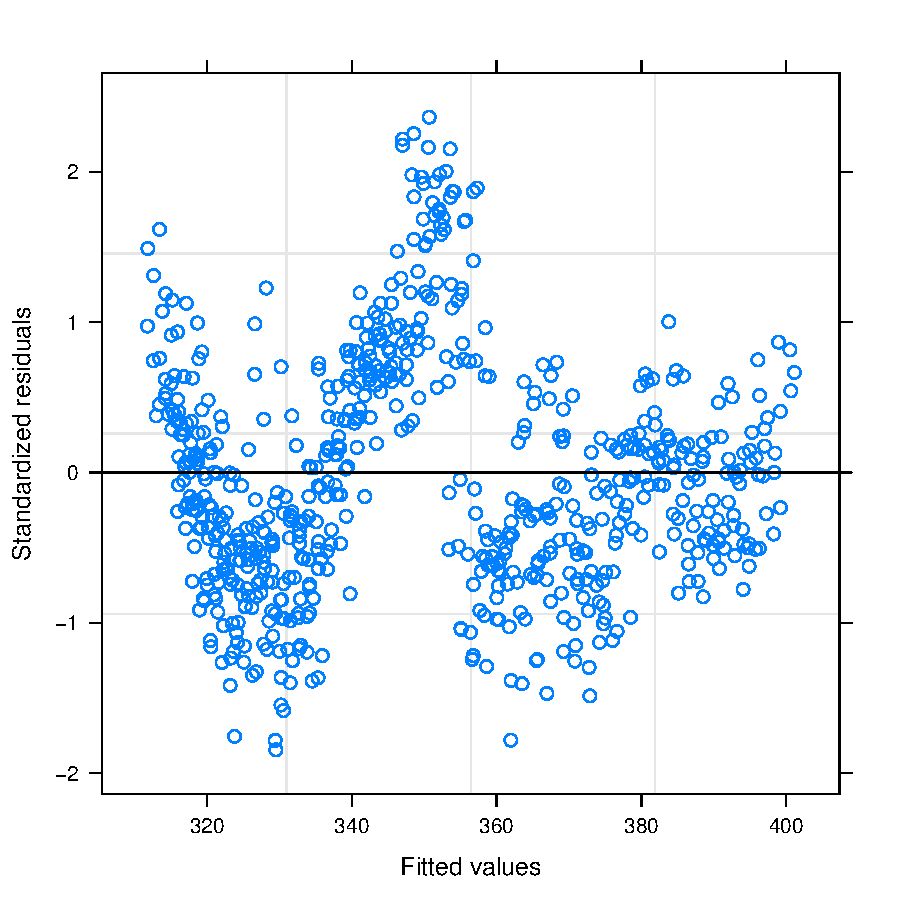
\includegraphics{alleselena-044}
\caption{Residuals fitted vs. obs. values ARMA harm.}
\label{comparison_finalgls3}
\end{figure}

\begin{Schunk}
\begin{Sinput}
> diagnostics(harmonizedARMAgls)
\end{Sinput}
\begin{Soutput}
     normality     stat.res   stat.res.alt
[1,] "5.22872e-08" "0.290355" "stationary"
     autocorr           indep
[1,] "0.18333304071156" "0"  
\end{Soutput}
\end{Schunk}

\begin{figure}[H]
\centering
\begin{Schunk}
\begin{Sinput}
> qqnorm(harmonizedARMAgls, abline=c(0,1))
\end{Sinput}
\end{Schunk}
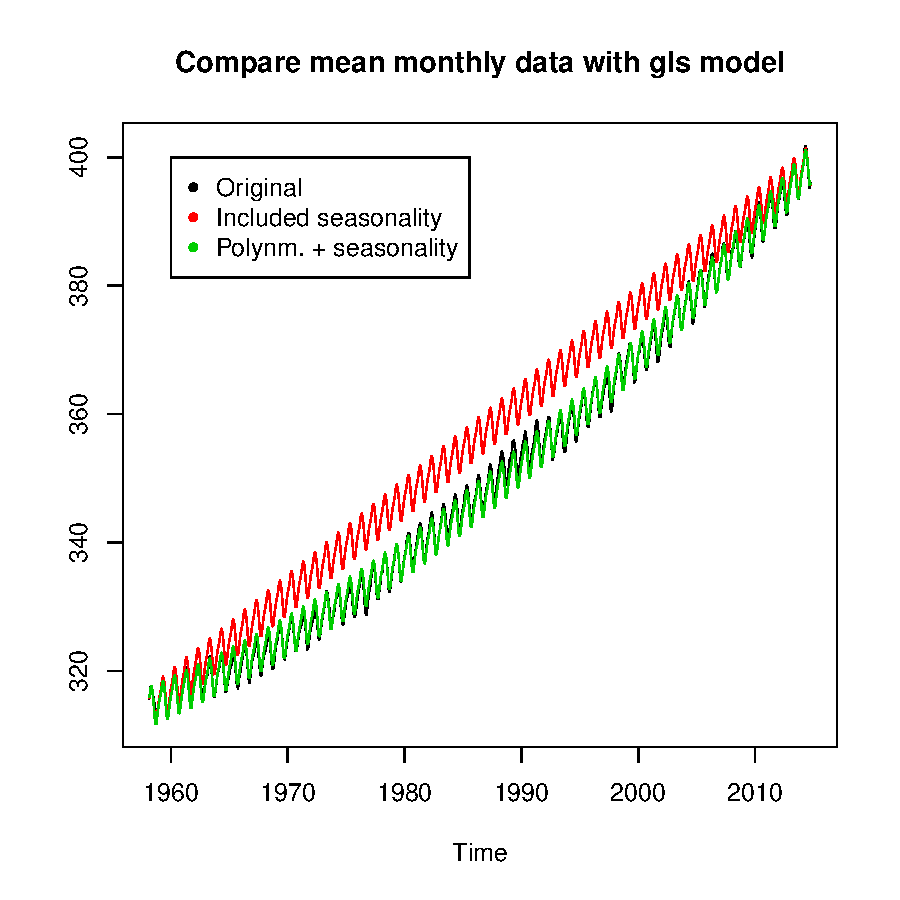
\includegraphics{alleselena-046}
\caption{look at norm. distribution}
\label{finalgls_norm}
\end{figure}

\linebreak
#bestmodel with smallest AIC: \\
\begin{Schunk}
\begin{Sinput}
> anova.all = anova( harmonizedgls,harmonizedARMAgls)
> #as.matrix(anova.all)
> bestmodel= anova.all$Model[anova.all$AIC ==min(anova.all$AIC)]
> bestmodel 
\end{Sinput}
\begin{Soutput}
[1] 2
\end{Soutput}
\begin{Sinput}
> #Our best model fitted by hand is the model: \Sexpr{bestmodel} ...
\end{Sinput}
\end{Schunk}

\begin{table}[ht]
\centering
\begin{tabular}{rlrrrrrlrr}
  \hline
 Model & df & AIC & BIC & logLik & Test & L.Ratio & p-value \\ 
  \hline
harmonizedgls  &    17 & 396.86 & 473.36 & -181.43 &  &  &  \\ 
  harmonizedARMAgls  &    20 & 360.41 & 450.40 & -160.20 & 1 vs 2 & 42.45 & 3.21739e$-$09 \\ 
   \hline
\end{tabular}
\end{table}

\linebreak

In the beginning we were talking about the underestimation of standard errors in the linear model, if not considering the autocorrelation. As we see, the standard errors are now less underestimated. 

\begin{Schunk}
\begin{Sinput}
> LM=sqrt(diag(vcov(datalm)))
> ARMA22=sqrt(diag(vcov(dataglsARMA22)))
> bestmodel=sqrt(diag(vcov(harmonizedARMAgls))[c(1,2)])
> SE = as.matrix(cbind(LM,ARMA22,bestmodel), byrow=T, nrow=2)
> xtable(SE)
\end{Sinput}
% latex table generated in R 3.1.1 by xtable 1.7-4 package
% Thu Nov 27 21:02:37 2014
\begin{table}[ht]
\centering
\begin{tabular}{rrrr}
  \hline
 & LM & ARMA22 & bestmodel \\ 
  \hline
(Intercept) & 16.98 & 45.71 & 4322.03 \\ 
  year & 0.01 & 0.02 & 4.35 \\ 
   \hline
\end{tabular}
\end{table}\end{Schunk}
\linebreak


\noindent After some trials to find the best gls model to our data, there are still some diagnostics failed. Our fitted values residuals are still not normally distributed, here you could think of normalizing them. Also the fitted values are still dependent, but our model seems not to care for this. A good result is, that the autocorrelation was solved and our model is now stationary (?)


\subsection{Modelling time series with ARIMA }
ARIMA modelling is a time efficient option to the gls(). 
The ARIMA function does not care about stationarity of the time series, it will adjust the model  to be stationary afterwards. 
The function auto.arima() will provide a dequately adjusted model with all needed components. 
\\


\begin{Schunk}
\begin{Sinput}
> autoarima = auto.arima(yourts)
\end{Sinput}
Series: yourts 
ARIMA(1,1,1)(2,1,2)[12]                    

Coefficients:
         ar1      ma1     sar1     sar2     sma1     sma2
      0.2166  -0.5763  -0.2861  -0.0364  -0.5992  -0.2292
s.e.  0.0936   0.0782      NaN   0.0404      NaN      NaN

sigma^2 estimated as 0.08927:  log likelihood=-149.46
AIC=312.92   AICc=313.09   BIC=344.44\begin{Sinput}
> print(autoarima)
\end{Sinput}
Series: yourts 
ARIMA(1,1,1)(2,1,2)[12]                    

Coefficients:
         ar1      ma1     sar1     sar2     sma1     sma2
      0.2166  -0.5763  -0.2861  -0.0364  -0.5992  -0.2292
s.e.  0.0936   0.0782      NaN   0.0404      NaN      NaN

sigma^2 estimated as 0.08927:  log likelihood=-149.46
AIC=312.92   AICc=313.09   BIC=344.44
Series: yourts 
ARIMA(1,1,1)(2,1,2)[12]                    

Coefficients:
         ar1      ma1     sar1     sar2     sma1     sma2
      0.2166  -0.5763  -0.2861  -0.0364  -0.5992  -0.2292
s.e.  0.0936   0.0782      NaN   0.0404      NaN      NaN

sigma^2 estimated as 0.08927:  log likelihood=-149.46
AIC=312.92   AICc=313.09   BIC=344.44\end{Schunk}

\begin{figure}[H]
\centering
\begin{Schunk}
\begin{Sinput}
> fitted=fitted(autoarima)
> par(mfrow=c(1,1))
> ts.plot(cbind(yourts, harmonizedARMAgls$fitted ), col=c(1,2,3))
> lines( fitted, col=3)
> legend(1960,400,c("Original",  "GLS", "Autoarima "),col=c(1,2,3), pch=c(20,20,20))
\end{Sinput}
\end{Schunk}
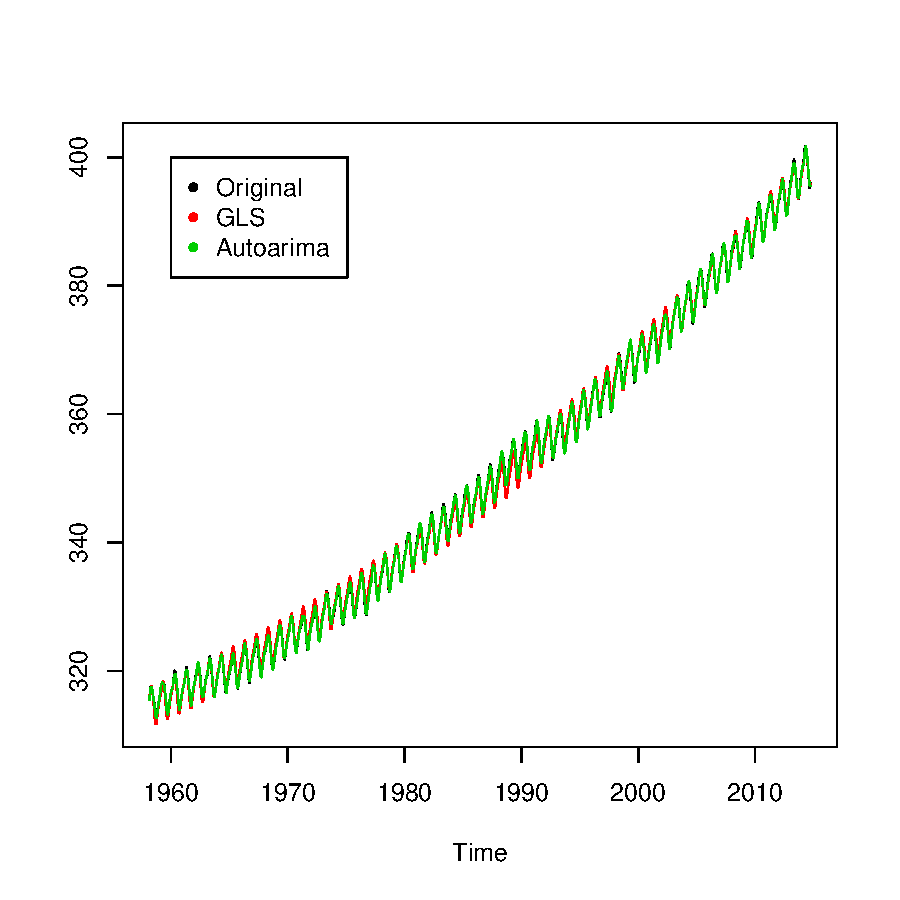
\includegraphics{alleselena-fittedarima}
\caption{Fitted ARIMA values on time series}
\label{fittedarima}
\end{figure}


The comparison plot ~/ref{fittedarima} shows that the bestmodel from gls() and the automatically adjusted arima model are barely distinguishable from the original dataset. However, the arima gives slightly better AIC than the best gls. 

\begin{Schunk}
\begin{Sinput}
> AIC(autoarima)
\end{Sinput}
[1] 312.9221\end{Schunk}

\begin{figure}[H]
\centering
\begin{Schunk}
\begin{Sinput}
> par(mfrow=c(3,1))
> acf(autoarima$residuals)
> pacf(autoarima$residuals)
> spectrum(autoarima$residuals)
\end{Sinput}
\end{Schunk}
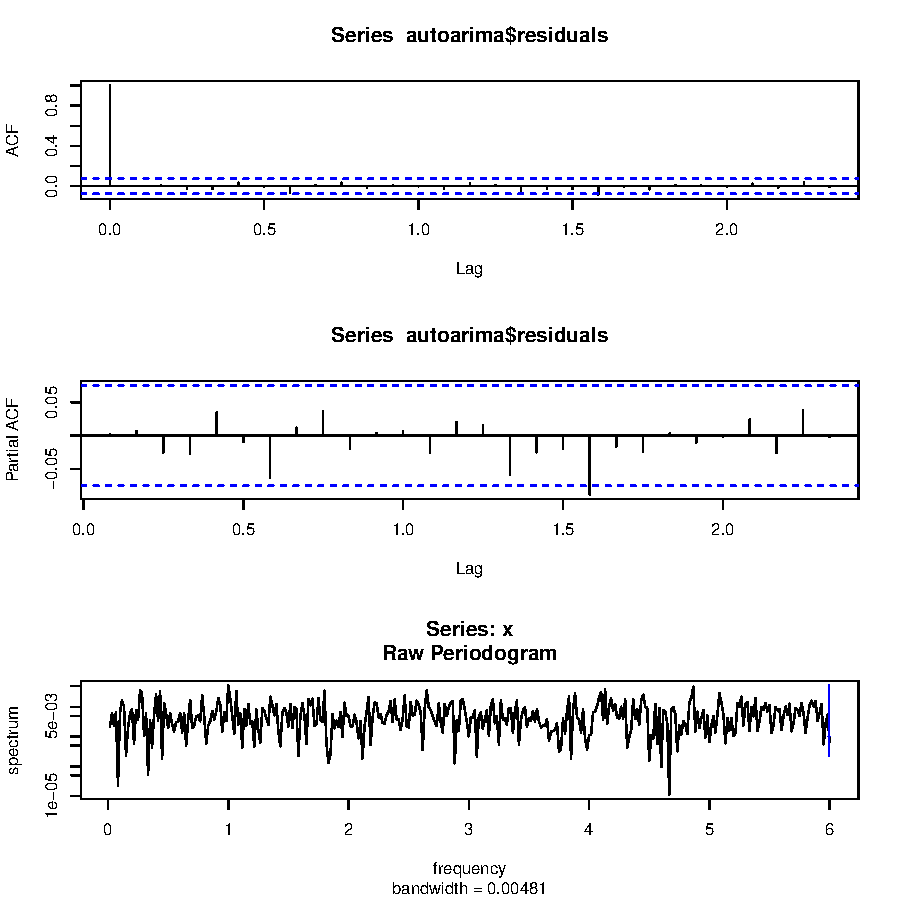
\includegraphics{alleselena-corarima}
\caption{Correlogram for ARIMA}
\label{corarima}
\end{figure}

\begin{figure}[H]
\centering
\begin{Schunk}
\begin{Sinput}
> qqnorm(autoarima$residuals)
> qqline(autoarima$residuals)
\end{Sinput}
\end{Schunk}
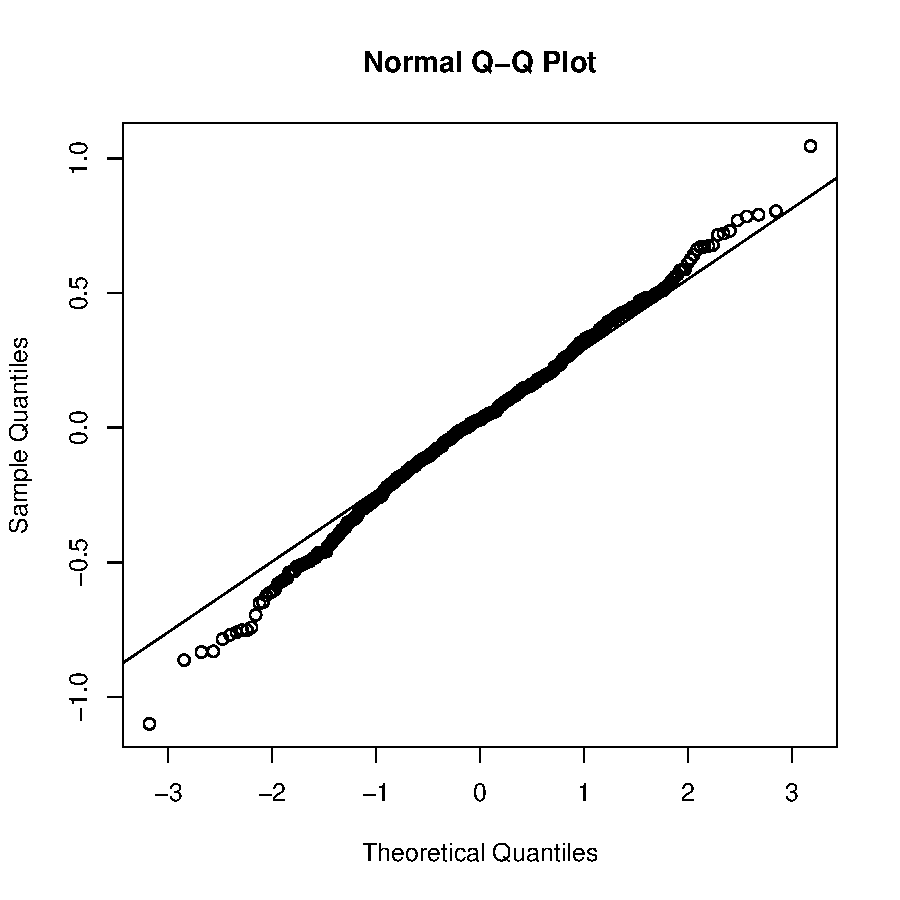
\includegraphics{alleselena-qqarima}
\caption{Correlogram for ARIMA}
\label{qqarima}
\end{figure}

diagnostics(autoarima)

The diagnostics show a better estimate of our fitted model. 
The autocorrelation is solved way better than in the gls-model. Also the stationarity is given now and the fitted values are independend. 



\section{Forecasts}%----------------------------------------------------------------------------------------------------
We have three different options to make ( up to now)
\begin{enumerate}
\item predict()
\item Holt Winters
\item Arima forecasts
\end{enumerate}

If we have a time series that can be described using an additive model,we can short-time forecast using exponential smoothing.\\
Preconditions: forecast errors are uncorrelated and are normally distributed with mean zero and constant variance. To check the forecast errors we have the visualization of the function from above. 

\subsection{Forecast with predict()}
We use our best gls model for this. 
\begin{Schunk}
\begin{Sinput}
> newtime= ts(start=c(2014, 10),end=c(2024,12),deltat=1/12)
> pred = predict(harmonizedARMAgls, newdata=newtime, se=T) 
> TIME <- as.numeric(time)
> time.df <- data.frame(TIME=TIME, COS, SIN)
> colnames(time.df)[-1] <- paste0("V", 1:12)
> smoothed <- gls(as.numeric(yourts) ~ TIME + I(TIME^2) + V1 + V2 + V3 + V4 + V5 
                 +V6 +V7+V8 +V9 +V10 +V11 +V12, 
                 corr=corAR1(acf(dataseasongls$residuals)$acf[2]),
                 data=time.df)
> new.df <- cbind.data.frame(TIME=as.numeric(time(newtime)), 
                            COS=COS[1:123,], SIN=SIN[1:123,])
> colnames(new.df)[-1] <- paste0("V", 1:12)
> pred = predictSE(smoothed, newdata=new.df, se.fit=T)
\end{Sinput}
\end{Schunk}

\begin{Schunk}
\begin{Sinput}
> plot(yourts, type="n",las=1, xlim=c(1960, 2025), 
      ylim=c(300, 450), xlab="Year", ylab="CO2 conc. (ppm)", 
      main="CO2 concentration in the atmosphere")
> grid (NULL,NULL, lty = 6, col = "cornsilk2") 
> points(yourts ,type="l" )
> par(mfrow=c(1,1))
> lines(as.numeric(time(newtime)), pred$fit, col="red")
> F=(pred$fit)
> FSUP=(pred$fit+1.96*pred$se.fit) # make upper conf. int. 
> FSLOW=(pred$fit-1.96*pred$se.fit) # make lower conf. int. 
> lines(new.df$TIME, FSUP,lty=1, col="grey", lwd=3)
> lines(new.df$TIME, FSLOW,lty=1, col="grey", lwd=3)
> lines(new.df$TIME, F, lty=1, col="red", lwd=1)
> legend("topleft",c("forecast for 10 years", "monthly mean data", "CI"), 
        pch=c(20,20), col=c("red", "black", "grey"))
\end{Sinput}
\end{Schunk}
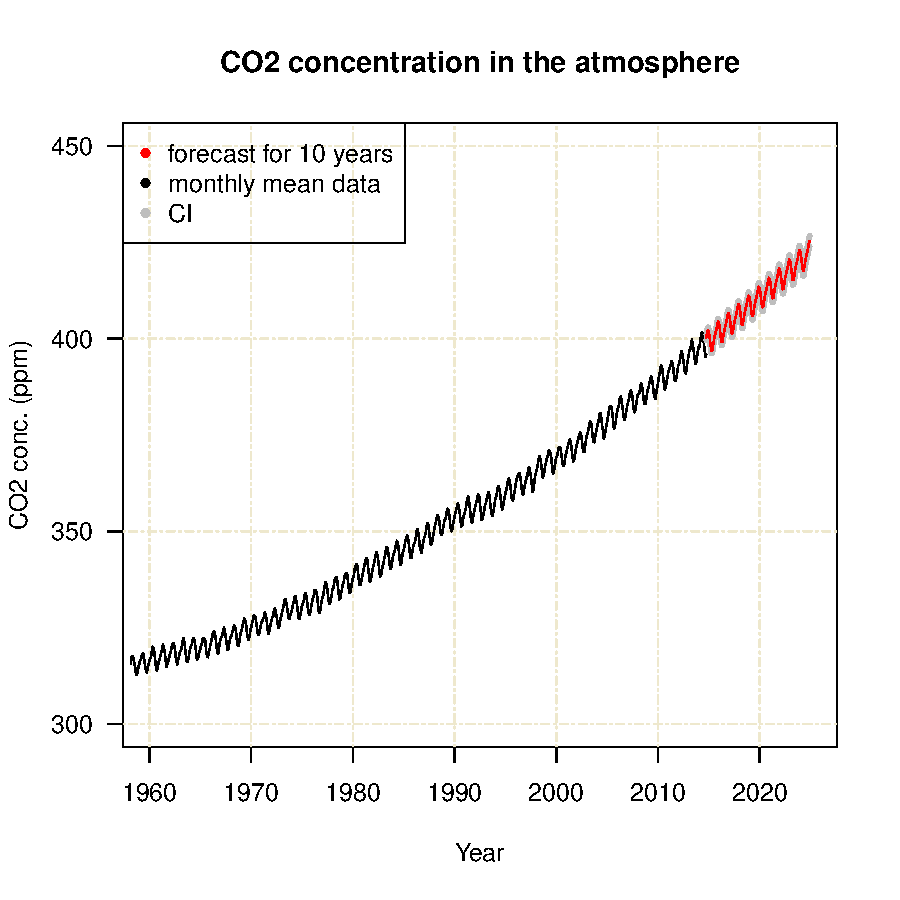
\includegraphics{alleselena-055}


\subsection{Holtwinters forecast function}
Forecasting: from past values (x1,x2,x3,...,xn) want to predict future values x(n+k), \\
holtwinters explanation: \\
#the alpha value tells us the weight of the previous values for the forecasting \\
#values of alpha that are close to 0 mean that little weight is placed on the most recent \\ observations when making forecasts of future values\\
#gamma is for the seasonality \\
if alpha is near 1, little smoothing, at is approx. xt \\
alpha is zero, highly smoothed estimates\\
a = 0.2 compromise figure, change in mean between t-1 and t likel smaller than variance\\

not specify aphla, beta, gamma to include errors, trend and seasonal component in the forecast\\
We use the original data for hw()\\
And predict in the period = 120* 1 month = 10 years\\
\begin{Schunk}
\begin{Sinput}
> forecast <- HoltWinters(yourts)
> forecast10 <- forecast.HoltWinters(forecast,h=120)
\end{Sinput}
\end{Schunk}

Lets see the plot\\
\begin{Schunk}
\begin{Sinput}
> par(mfrow=c(1,1))
> plot.forecast(forecast10,shadecols = "oldstyle")
\end{Sinput}
\end{Schunk}
check for the autocorrelation of the future values\\
\begin{Schunk}
\begin{Sinput}
> par(mfrow=c(2,1))
> acf(forecast10$residuals)
> pacf(forecast10$residuals)
\end{Sinput}
\end{Schunk}
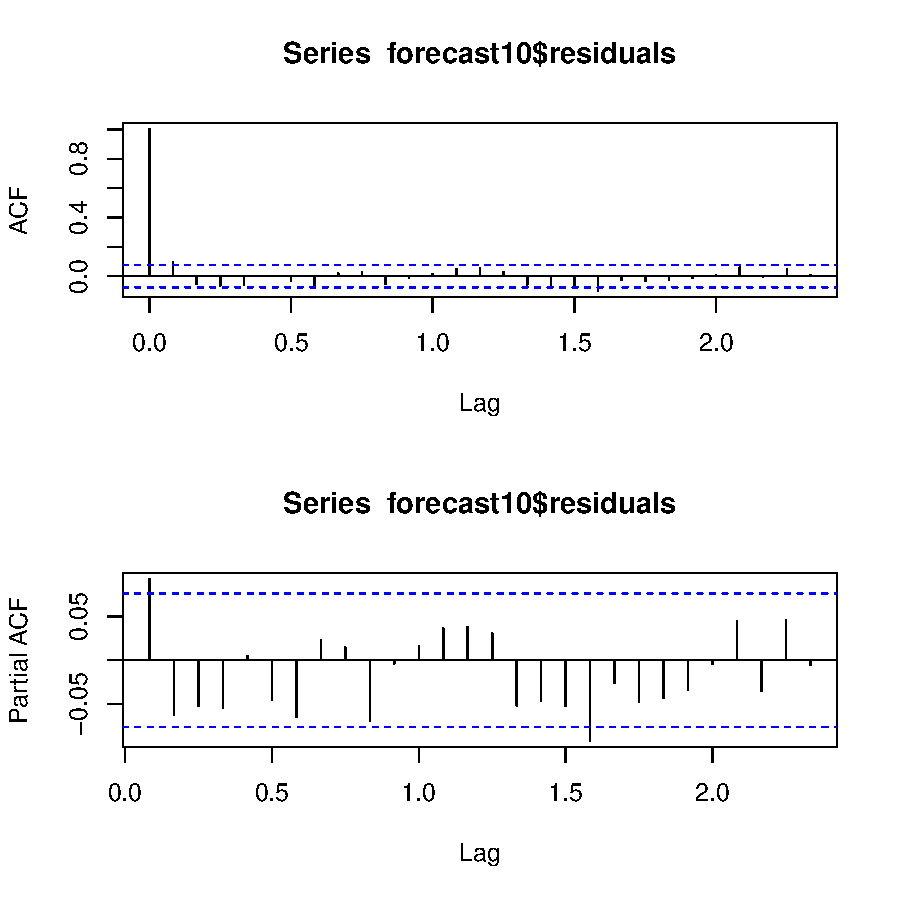
\includegraphics{alleselena-058}
and do the diagnostics on it\\
\begin{Schunk}
\begin{Sinput}
> list = as.list(diagnostics(forecast10))
> print(list)
\end{Sinput}
[[1]]
[1] "0.357443"

[[2]]
[1] "0.01"

[[3]]
[1] "stationary"

[[4]]
[1] "1.80314031521739"

[[5]]
[1] "0.0174092"\end{Schunk}

\subsection{ARIMA forecast function}
Now we try to forecast with the autoarima function as our bestmodel, which would save alot of time. 

\begin{Schunk}
\begin{Sinput}
> forecast.arima = forecast.Arima(autoarima, h=120) 
\end{Sinput}
\end{Schunk}

\subsection{Comparison of HW and ARIMA}
Lets compare what it better. 

\begin{Schunk}
\begin{Sinput}
> par(mfrow=c(2,1))
> plot.forecast(forecast.arima)
> plot.forecast(forecast10)
\end{Sinput}
\end{Schunk}
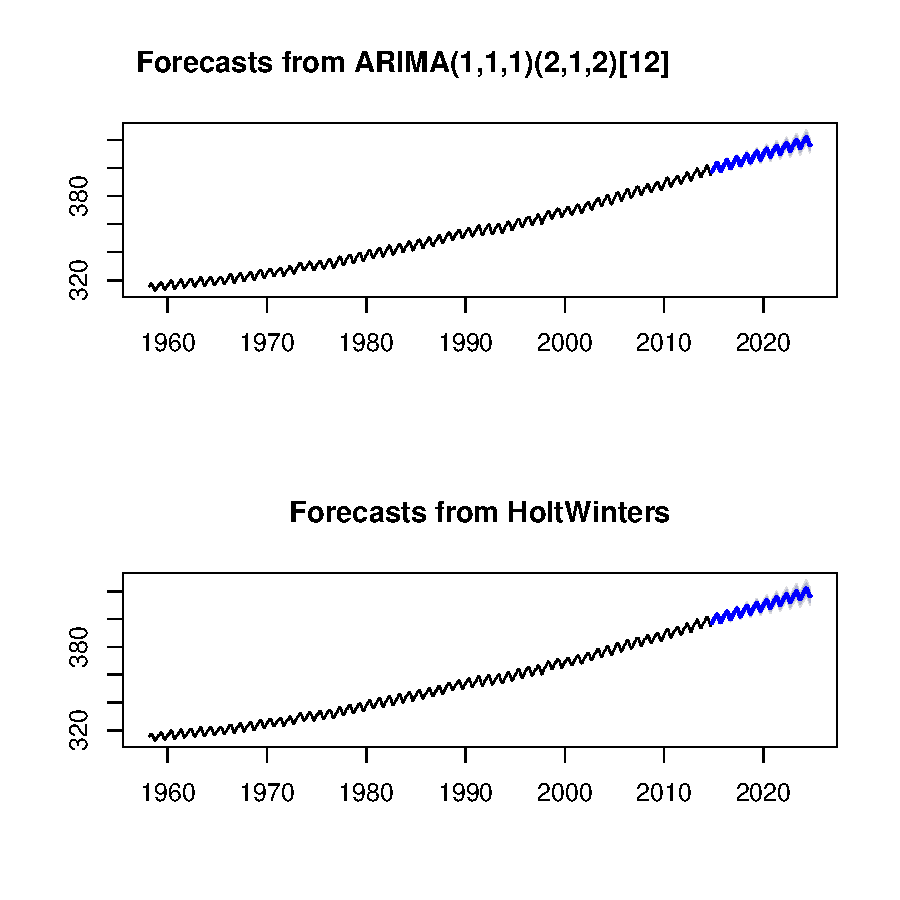
\includegraphics{alleselena-061}

#check for error distirbution with the plotForecastErrors function from above 
\begin{Schunk}
\begin{Sinput}
> par(mfrow=c(1,2))
> plotForecastErrors(forecast10$residuals)
> plotForecastErrors(forecast.arima$residuals)
\end{Sinput}
\end{Schunk}
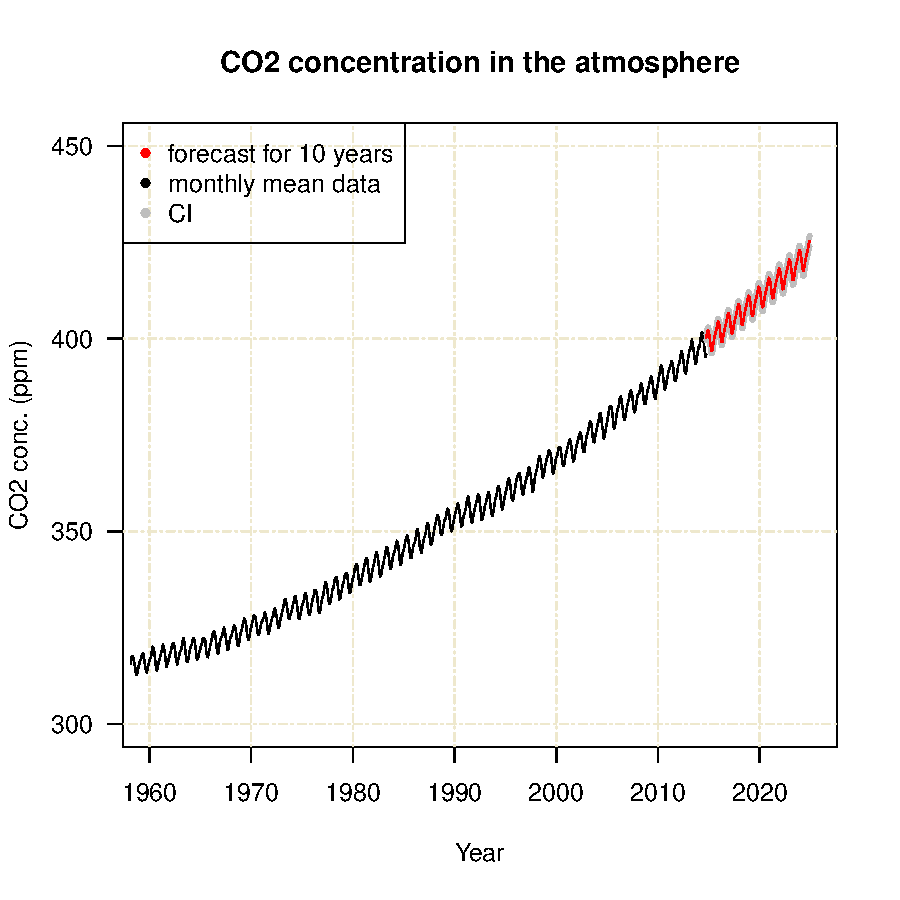
\includegraphics{alleselena-062}
\noindent The histogram of the time series shows that the forecast errors are roughly normally distributed and the mean seems to be close to zero.\\

run diagnostics
\begin{Schunk}
\begin{Sinput}
> list1= as.list(diagnostics(forecast10))
> (list1)
\end{Sinput}
\begin{Soutput}
[[1]]
[1] "0.357443"

[[2]]
[1] "0.01"

[[3]]
[1] "stationary"

[[4]]
[1] "1.80314031521739"

[[5]]
[1] "0.0174092"
\end{Soutput}
\begin{Sinput}
> list2= as.list(diagnostics(forecast.arima))
> (list2)
\end{Sinput}
\begin{Soutput}
[[1]]
[1] "0.037855"

[[2]]
[1] "0.01"

[[3]]
[1] "stationary"

[[4]]
[1] "1.97955655809946"

[[5]]
[1] "0.946122"
\end{Soutput}
\end{Schunk}
\linebreak
look at both zoomed in forecasts:
\begin{Schunk}
\begin{Sinput}
> par(mfrow=c(1,2))
> plot(forecast.arima, xlim=c(2010,2025), ylim=c(385,430),shadecols = "oldstyle")
> plot.forecast(forecast10 ,xlim=c(2010,2025), ylim=c(385,430),shadecols = "oldstyle")
\end{Sinput}
\end{Schunk}
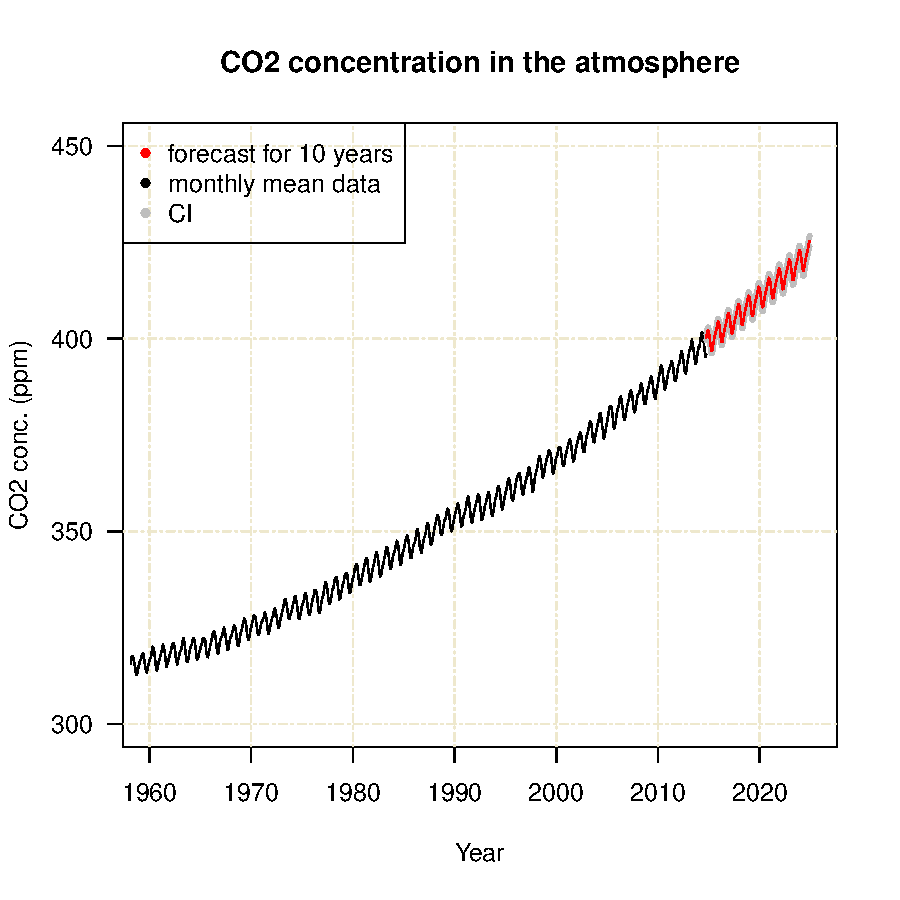
\includegraphics{alleselena-064}



\subsection{Seasonal Decomposition of Time Series by Loess}

Forecasting using stl objects:
\begin{figure}[H]
\centering
\begin{Schunk}
\begin{Sinput}
> plot(stlf(yourts, lambda=0, h =120))
> (tslm(yourts~time(yourts)))
\end{Sinput}
\begin{Soutput}
Call:
lm(formula = formula, data = "yourts", na.action = na.exclude)

Coefficients:
 (Intercept)  time(yourts)  
   -2618.494         1.494  
\end{Soutput}
\end{Schunk}
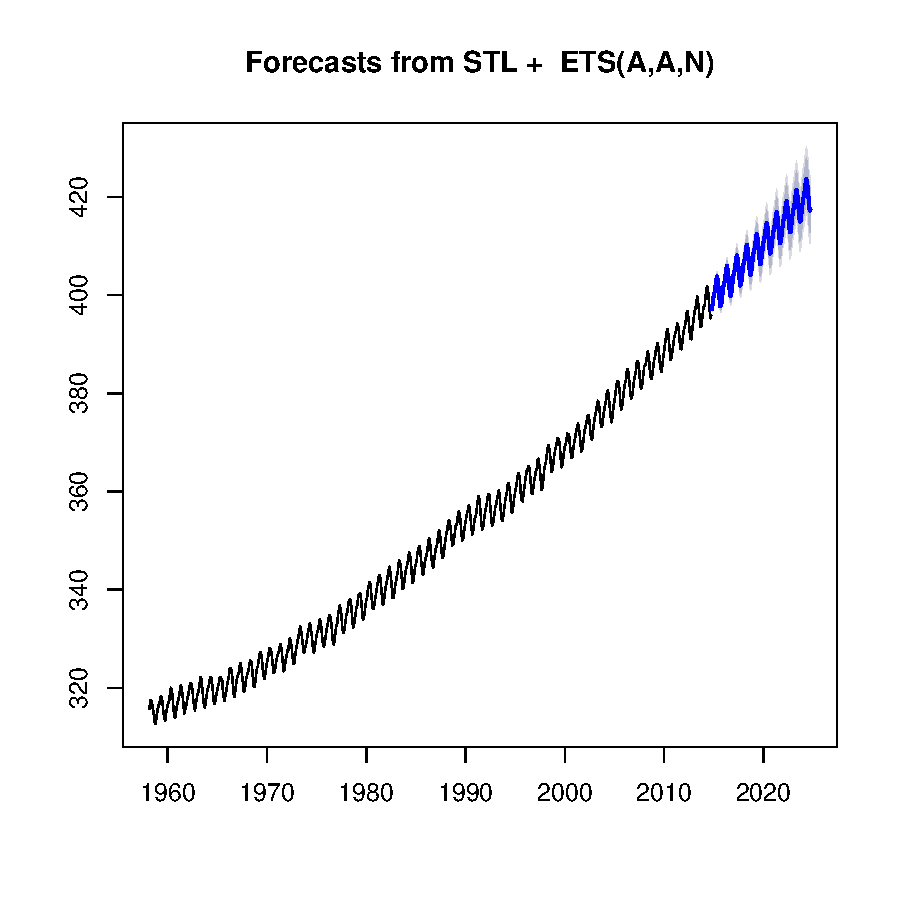
\includegraphics{alleselena-065}
\caption{Forecasting using Loess}
\end{figure}




\section{compabitily with Linux and Windows when working together on a sweave document.}
If you have Linux and have problems working on a same sweave document with Windows users because the line breaks and other text configurations are different, try to type:


\section{Links and Further Reading}%-----------------------------------------------------------------------------------------------


\subsection{Modelling time series with gam}

The gam() generalized additive model could maybe also help finding a quick solution for time series modelling. 

\begin{Schunk}
\begin{Sinput}
> model = gam ( yourts ~ s(time))
> summary(model)
\end{Sinput}
Family: gaussian 
Link function: identity 

Formula:
yourts ~ s(time)

Parametric coefficients:
             Estimate Std. Error t value Pr(>|t|)    
(Intercept) 350.09641    0.08181    4279   <2e-16 ***
---
Signif. codes:  
0 '***' 0.001 '**' 0.01 '*' 0.05 '.' 0.1 ' ' 1

Approximate significance of smooth terms:
          edf Ref.df     F p-value    
s(time) 6.969  8.047 11258  <2e-16 ***
---
Signif. codes:  
0 '***' 0.001 '**' 0.01 '*' 0.05 '.' 0.1 ' ' 1

R-sq.(adj) =  0.993   Deviance explained = 99.3%
GCV = 4.6049  Scale est. = 4.551     n = 680\end{Schunk}

\begin{Schunk}
\begin{Sinput}
> par(mfrow=c(1,1))
> plot.gam(model, residuals=T, scheme=c(2,1), all.terms=T)
\end{Sinput}
\end{Schunk}
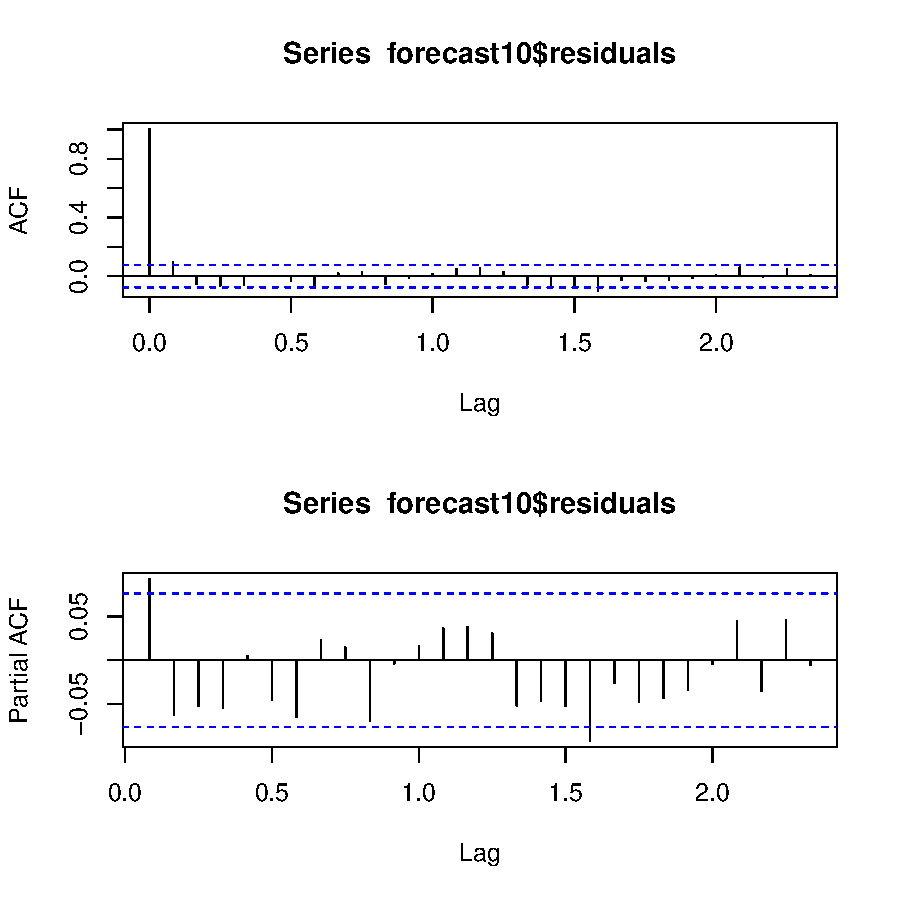
\includegraphics{alleselena-067}

\begin{Schunk}
\begin{Sinput}
> smoothed4gam <- gam(as.numeric(yourts) ~ s(time)  +
                         COS[,1]+SIN[,1]+COS[,2]+SIN[,2]+
                         COS[,3]+SIN[,3]+COS[,4]+SIN[,4]+
                         COS[,5]+SIN[,5]+COS[,6]+SIN[,6]
                       , cor=corARMA(p=2, q=2))
> #summary(smoothed4gam)
> AIC(smoothed4gam)
\end{Sinput}
[1] 926.9626\end{Schunk}

\begin{Schunk}
\begin{Sinput}
> plot(smoothed4gam)
> #8.91 is the edf:array of estimated degrees of freedom for the model terms, calculated for the smoothing term s(time)
\end{Sinput}
\end{Schunk}
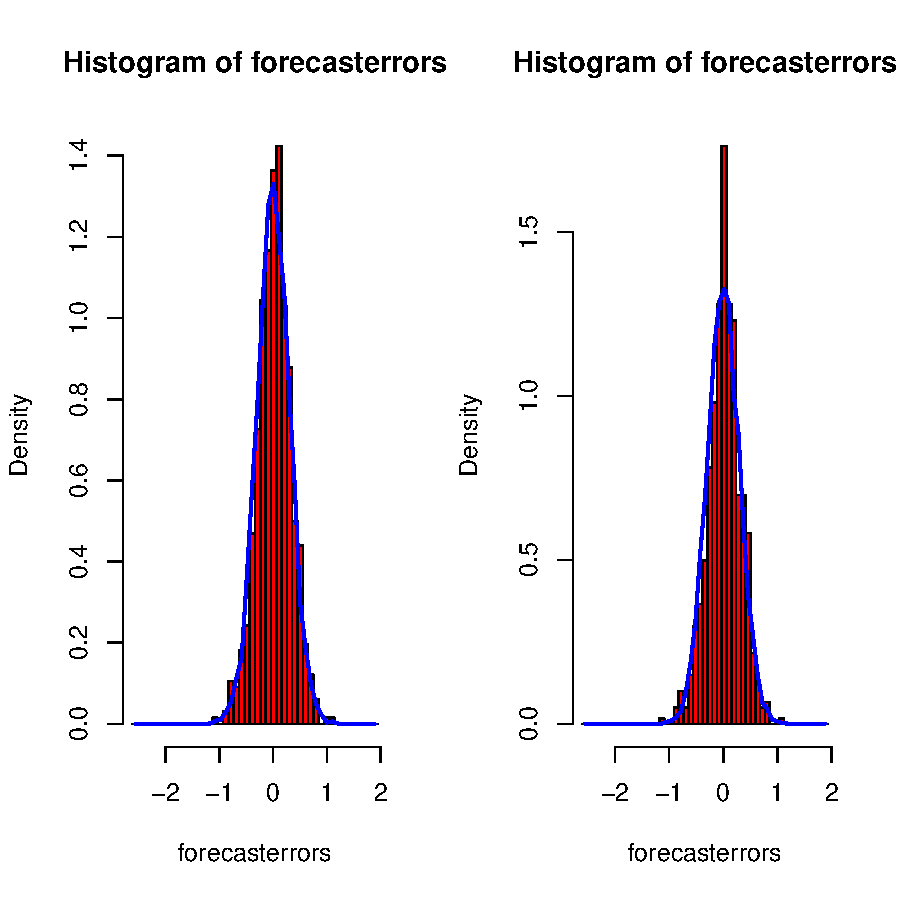
\includegraphics{alleselena-069}

Thus this model is not adequately adjusted there are examples for modelling also seasonally components with gam(). 

Example: 


and in:\\
http://cran.r-project.org/web/views/TimeSeries.html\\
Another Exemple Datasets are avaliable at:\\
http://www.comp-engine.org/timeseries/browse-data-by-category\\
https://datamarket.com/data/list/?q=provider:tsdl\\
\section{Acknowledgements}%------------------------------------------------------------------------------------------------------
Don't forget to thank TeX and R and other opensource communities if you use their products! The correct way to cite R is shown when typing ``\texttt{citation()}'', and ``\texttt{citation("mgcv")}'' for packages.

\clearpage
\end{document}
